\documentclass[12pt]{article}
\usepackage[spanish]{babel}
\usepackage{graphicx}
\usepackage{amsmath} 
\usepackage{placeins}
\usepackage{hyperref}
\usepackage[margin=1.2in]{geometry}
\usepackage{multirow}
\usepackage{float}
\usepackage{subcaption}

\title{Visión Artificial Avanzada - Trabajo Práctico II}
\author{Manuel Ramirez Silva y Felipe Laffaye}
\date{}
\begin{document}

\maketitle

\section{Introducción}
Una de las maneras más populares y efectivas de entrenar un modelo de deep learning es a través de la supervisión. Usar datos para estimar cómo deben ajustarse los parámetros de la red para minimizar una función de costo es una estrategia que funciona muy bien. Pero para eso necesitamos tener datos. No siempre va a ser fácil conseguir los datos que necesitamos para la tarea que queremos que el modelo aprenda a resolver. También hay casos en los cuales tenemos acceso a datos, pero el modelo o la tarea son extremadamente complejos, y requieren un volumen de datos que no tenemos. El paradigma de meta-learning se propone atacar este problema y lograr que un modelo pueda aprender rápidamente una nueva tarea con pocos datos. En otras palabras, los métodos de meta-learning aprenden a aprender.

Un caso partícular de aprender a resolver una nueva tarea es que la tarea en sí no cambie, pero el dominio sí. Esto es lo que se va a estar trabajando. La tarea será siempre la misma: determinar correctamente qué digito está presente en una imagen. Sin embargo, el dominio de las imágenes cambiará. Se trabajará con tres datasets: el MNIST, el MNIST-M y el SVHN. Cada uno de ellos representa un dominio distinto para la misma tarea. Sobre estos dominios se implementarán tres métodos de meta-learning: Prototypical Networks (ProtoNets), MAML (Model-Agnostic Meta-Learning) y Proto-MAML. Estos métodos serán entrenados en solo uno de los dominios: el MNIST; y luego se evaluará su capacidad de aprender rápidamente a clasificar las imágenes de los otros dos dominios. Luego, se implementará DANN (Domain-Adversarial-Neural-Network), un método diseñado específicamente para la adaptación de dominios. Este método se entrenará con datos del dominio MNIST-M, pero sin etiquetas.

En la siguiente sección se explicará más en detalle cómo funciona cada método, qué decisiones se tomó para implementar cada uno y qué hiperparámetros se usó. Luego, habrá una sección de resultados en la cual se expondrá cómo se desempeñó cada método.

\section{Métodos implementados}

Antes de discutir los métodos en sí, es importante entender cómo funciona el meta-training. En el aprendizaje supervisado clásico, tenemos $X$ clases en nuestro dataset y tomamos un batch de $K$ muestras para cada paso de gradiente descendente. En el batch que muestreamos puede haber muestras de todas las clases. En cambio, en el meta-trainig, usamos episodios N-way K-shot. $N$ corresponde a la cantidad de clases de las cuales muestreamos ($N < X$), mientras que $K$ indica cuántas muestras tomamos de cada clase. La gracia del entrenamiento episódico es que emula la situación en la que se encontrará el modelo a la hora de aprender una nueva tarea: nuevas clases y pocas muestras. Por último, una epoch de entrenamiento lleva a cabo múltiples episodios para constuir una señal de entrenamiento más robusta y que no esté condicionada por un solo episodio y sus clases.

Habiendo dicho eso, el primer método que implementamos fue ProtoNets. Este método consiste de solamente un encoder. No hay una cabeza de clasificación involucrada, sino que la clasificación ocurre directamente en el espacio latente. Para un episodio N-way K-shot, se pasa cada muestra por el encoder para obtener su embedding. Luego, se toma el promedio de los embeddings de cada clase. A ese promedio se lo llama el prototipo de la clase para ese episodio. Luego, el episodio va acompañado de $Q$ muestras adicionales (el query set). A esas muestras también se las pasa por el encoder, y luego se las compara con los prototipos. Se toma la función softmax de las distancias negativas entre la query y cada prototipo. Esa es la estimación del modelo de cuán probable es que la query $q$ pertenezca a cada clase.

\begin{equation}
    p(y = n \mid \mathbf{q}) = \frac{\exp(-d(\mathbf{f}_\phi(\mathbf{q}),\, \mathbf{c}_n))}{\sum_{n'} \exp(-d(\mathbf{f}_\phi(\mathbf{q}),\, \mathbf{c}_{n'}))}
\end{equation}

Luego, se utiliza la pérdida de entropía cruzada como objetivo de entrenamiento. 


\begin{equation}
\mathcal{L} = -\log p(y = n^* \mid \mathbf{x})
\end{equation}

Esto significa que cuanto menor distancia haya entre una query y el prototipo de su clase, menor será la pérdida. Por lo cual la ProtoNet aprende a construir un espacio latente en el cual las muestras de la misma clase están juntas, mientras que las muestras de clases distintas se separan.

En cuanto a la red en sí, utilizamos una CNN básica con cuatro capas. Elegimos usar convoluciones en dos dimensiones porque estas son buenas capturando información espacial y relaciones entre píxeles. Usamos una arquitectura sencilla por la naturaleza simple y de baja dimensionalidad de los datos (las imágenes de MNIST y MNIST-M son de $28 \times 28$ y las de SVHN son de $32 \times 32$). Cada capa tiene una convolución con un kernel de tamaño $3 \times 3$, una función de activación ReLU y un max pooling de $2 \times 2$. La cantidad de canales por capa es 64, por lo cual la red devuelve un embedding de 64 dimensiones. Elegimos 64 dimensiones porque consideramos que sería suficiente dado que estamos trabajando con imágenes sencillas y de muy baja resolución.

Para entrenar nuestra red, llevamos a cabo episodios 5-way, 5-shot e incluímos un query set de tamaño 15 en cada episodio. Más allá de que lo haya pedido la consigna explícitamente, consideramos que 5 es un buen número para $N$ porque si $N$ es muy alto (cerca de 10), no permite tanto que cada episodio tenga distintas clases. Esto no es bueno porque queremos que el modelo se acostumbre a ver clases distintas en cada episodio. De esta forma, estará más preparado para encontrarse con clases o dominios nuevos después del entrenamiento. Si $N$ es demasiado bajo (cerca de 1), es demasiado fácil que el modelo clasifique las queries correctamente a pesar de haber formado representaciones latentes malas. Esto haría que la señal de entrenamiento se vuelva muy ruidosa y se dificulte el entrenamiento del modelo. Por eso el número 5 es un buen punto medio.

En cuanto a hiperparámetros y configuraciones de entrenamiento, realizamos un \textit{grid search} y nos quedamos con la configuración que mejores resultados nos trajo, resumida en la Tabla~\ref{tab:hp_protonet}.

\begin{table}[h]
    \centering
    \begin{tabular}{ll}
        \hline
        Hiperparámetro                       & Valor          \\
        \hline
        Episodios                            & 5-way 5-shot   \\
        Query set por episodio ($Q$)         & 15             \\
        Episodios de entrenamiento por época & 10             \\
        Episodios de validación por época    & 10             \\
        Épocas                               & 20             \\
        Optimizador                          & Adam           \\
        \textit{Learning rate} inicial       & $10^{-3}$      \\
        \textit{Step decay} del \textit{lr}  & $\gamma=0.5$ cada 10 épocas \\
        Dimensión del \textit{embedding} (\textit{hidden\_dim}) & 64 \\
        \textit{Seed}                        & 42             \\
        \hline
    \end{tabular}
    \caption{Hiperparámetros utilizados para entrenar ProtoNet sobre MNIST.}
    \label{tab:hp_protonet}
\end{table}

La Tabla~\ref{tab:gs_protonet} muestra los valores que exploramos en el \textit{grid search} para cada hiperparámetro. Mantuvimos fijos $N=5$ (sugerido por la consigna), $K=5$ y $Q=15$, y barrimos los ejes restantes (lr, decaimiento, dimensión del \textit{embedding} y número de épocas).

\begin{table}[H]
    \centering
    \begin{tabular}{ll}
        \hline
        Hiperparámetro                       & Valores explorados \\
        \hline
        Épocas                               & $\{10, 20, 50\}$ \\
        Episodios de entrenamiento por época & $\{10, 50, 100\}$ \\
        \textit{Learning rate} inicial       & $\{10^{-4}, 5 \cdot 10^{-4}, 10^{-3}, 5 \cdot 10^{-3}\}$ \\
        \textit{lr\_step} (período del \textit{step decay}) & $\{5, 10, 20\}$ \\
        \textit{lr\_gamma} (factor del \textit{step decay}) & $\{0.1, 0.5, 1.0\}$ \\
        Dimensión del \textit{embedding} (\textit{hidden\_dim}) & $\{32, 64, 128\}$ \\
        \hline
    \end{tabular}
    \caption{Espacio de búsqueda explorado en el \textit{grid search} de ProtoNet. La configuración ganadora se reporta en la Tabla~\ref{tab:hp_protonet}.}
    \label{tab:gs_protonet}
\end{table}

\section{MAML}

El método MAML propone hallar un conjunto de parámetros tales que el modelo pueda adaptarse a una nueva tarea con pocos pasos de gradiente descendente (y por ende con pocos datos). El objetivo de entrenamiento de MAML no es maximizar el desempeño sobre una tarea, sino facilitar lo más posible el fine-tuneo a una nueva tarea.

El entrenamiento de MAML se divide en dos partes: el bucle externo y el interno. En el bucle interno se trabaja con una sola tarea y algunas muestras de esa tarea. Se entrena al modelo para minimizar la pérdida específica de esa tarea realizando unos pocos pasos de gradiente descendente con las muestras disponibles. Luego, se almacenan los parámetros obtenidos tras la optimización para ser utilizados en el bucle externo. Los verdaderos parámetros del modelo no se actualizan definitivamente hasta realizar el bucle externo.

Una vez obtenidos los parámetros optimizados para cada tarea con la que se está trabajando, se avanza al bucle externo. En este bucle, sí se actualizan definitivamente los parametros del modelo. Para hacerlo, se construye una función de pérdida a partir de los parámetros obtenidos en los bucles internos para las distintas tareas y un query set para cada tarea.

\begin{equation}
    \mathcal{L} = \sum_{T_i \sim p(T)} \mathcal{L}_{T_i}(f_{\theta'_i}, q_i)
\end{equation}

Donde $T_i$ es una tarea, $\mathcal{L}_{T_i}$ es la función de pérdida para esa tarea, y $f_{\theta'_i}$ es el modelo con los parámetros $\theta'_i$ aprendidos en el bucle interno de esa tarea. Entonces en definitiva lo que hace MAML es hallar un conjunto de parámetros para el cual se minimice la suma de las pérdidas de un conjunto de tareas distintas. De esta forma, no se logra desempeño óptimo en ninguna, pero se puede alcanzarlo con pocos pasos de gradiente descendente y pocos datos. Para minimizar esta pérdida compuesta de otras pérdidas, es necesario tomar un gradiente de segundo orden.

\begin{equation}
    \nabla_\theta \mathcal{L}_{T_i}(\theta'_i) = \nabla_\theta \mathcal{L}_{T_i}\!\left(\theta - \alpha \nabla_\theta \mathcal{L}_{T_i}(\theta)\right)
\end{equation}

La ecuación (4) describe cómo deben ajustarse los pesos $\theta$ de la red para minimizar la pérdida de la tarea $T_i$ bajo los parámetros $\theta'$. Luego se suman todos los gradientes de segundo orden (uno para cada tarea) y se obtiene el gradiente total que minimiza la suma de las pérdidas de cada tarea.

En cuanto a la implementación, entrenamos con episodios 5-way 1-shot y 15 muestras en el query set. Utilizamos la misma arquitectura para el encoder que la que usamos para ProtoNets. Lo hicimos por las mismas razones que dimos para ProtoNets: las imágenes con las que estamos trabajando son simples y de baja dimensionalidad, y no se necesita más que algunas capas convolucionales con sus no-linealidades y MaxPoolings para alcanzar buenas representaciones latentes de las imágenes. Después del encoder colocamos una cabeza de clasificación lineal con $N$ salidas (una por cada clase del episodio, $N=5$ durante el entrenamiento). Recibe como entrada el embedding de 64 dimensiones del encoder y lo pasa por una sola capa lineal a cuyas activaciones se les aplica la función softmax para obtener las probabilidades de cada clase. En un principio pensamos que tener una capa adicional intermedia sería mejor, ya que introduciría una instancia de no-linealidad y mejoraría la expresividad de la cabeza de clasificación. Pero al probar ambas opciones obtuvimos prácticamente los mismos resultados, por lo cual decidimos quedarnos con una única capa lineal ya que es más liviano y rápido de entrenar y evaluar. Como la cabeza es específica de cada episodio, la dejamos depender del $N$ del episodio: durante el entrenamiento se reinicializa con cada batch de tareas y al evaluar en test con $N=10$ se reinicializa también con esa dimensión (aleatoriamente para MAML, según los prototipos en el caso de ProtoMAML). El encoder es lo único que persiste entre episodios.

Para poder tomar un gradiente de segundo orden, hicimos que pytorch almacene en el grafo computacional los gradientes calculados en el bucle interno en vez de descartarlos. Esto se hace utilizando

\begin{verbatim}
grads = torch.autograd.grad(
    loss,
    adapted.values(),
    create_graph=True,
    
)    
\end{verbatim}

En particular, la línea create\_graph=True es la responsable por conservar los gradientes calculados en el grafo computacional. Luego, a la hora de calcular la pérdida para una tarea, es importante utilizar las salidas del modelo bajo los parámetros $\theta'$ adaptados para esa tarea y no los parámetros $\theta$ actuales del modelo.

En este trabajo, no entrenamos al modelo utilizando tareas verdaderamente distintas. Semánticamente, la tarea de entrenamiento fue siempre la misma y en el mismo dominio: identificar qué número está escrito en una imagen de MNIST. Sin embargo, en cada episodio de entrenamiento, el modelo ve cinco clases distintas. Clasificar entre las clases 1, 2, 3, 4 y 5 es una tarea distinta que hacerlo para las clases 3, 4, 5, 6, y 7 por ejemplo. Y esa es la noción de tarea bajo la cual trabajamos.

Al igual que con ProtoNets, realizamos un \textit{grid search} para hallar hiperparámetros. La configuración con la que obtuvimos los mejores resultados está resumida en la Tabla~\ref{tab:hp_maml}.

\begin{table}[h]
    \centering
    \begin{tabular}{ll}
        \hline
        Hiperparámetro                       & Valor          \\
        \hline
        Episodios                            & 5-way 1-shot   \\
        Query set por episodio ($Q$)         & 15             \\
        Episodios de entrenamiento por época & 50             \\
        Episodios de validación por época    & 50             \\
        Épocas                               & 50             \\
        \textit{Inner loop} — \textit{learning rate}    & $10^{-2}$ \\
        \textit{Inner loop} — pasos de gradiente        & 5         \\
        \textit{Outer loop} — optimizador               & Adam      \\
        \textit{Outer loop} — \textit{learning rate}    & $10^{-3}$ \\
        Dimensión del \textit{embedding} (\textit{hidden\_dim}) & 64 \\
        \textit{Seed}                        & 42             \\
        \hline
    \end{tabular}
    \caption{Hiperparámetros utilizados para entrenar MAML sobre MNIST.}
    \label{tab:hp_maml}
\end{table}

La Tabla~\ref{tab:gs_maml} resume los valores explorados en el \textit{grid search} de MAML. Mantuvimos $N=5$, $K=1$ y $Q=15$ fijos (configuración típica de MAML en literatura para evaluar few-shot), y barrimos los ejes restantes: el \textit{learning rate} de los dos bucles, la cantidad de pasos del \textit{inner loop}, la cantidad de episodios por época y la dimensión del \textit{embedding}.

\begin{table}[H]
    \centering
    \begin{tabular}{ll}
        \hline
        Hiperparámetro                                   & Valores explorados \\
        \hline
        Épocas                                           & $\{30, 50, 100\}$ \\
        Episodios de entrenamiento por época             & $\{50, 100, 200\}$ \\
        \textit{Inner loop} — \textit{learning rate}     & $\{10^{-3}, 5 \cdot 10^{-3}, 10^{-2}, 5 \cdot 10^{-2}\}$ \\
        \textit{Inner loop} — pasos de gradiente         & $\{1, 3, 5, 10\}$ \\
        \textit{Outer loop} — \textit{learning rate}     & $\{10^{-4}, 5 \cdot 10^{-4}, 10^{-3}, 5 \cdot 10^{-3}\}$ \\
        Dimensión del \textit{embedding} (\textit{hidden\_dim}) & $\{32, 64, 128\}$ \\
        \hline
    \end{tabular}
    \caption{Espacio de búsqueda explorado en el \textit{grid search} de MAML. La configuración ganadora se reporta en la Tabla~\ref{tab:hp_maml}.}
    \label{tab:gs_maml}
\end{table}

\section{ProtoMAML}

ProtoMAML (Triantafillou et al., 2020) es una mejora de MAML que utiliza la noción de prototipos (al igual que ProtoNets) para inicializar inteligentemente la cabeza de clasificación. Sus autores notaron que, dados los prototipos $v_c$ del support set (las salidas promedio del encoder por clase $c$), si se inicializa la fila $c$ de la matriz de pesos como $W_c = 2\,v_c^\top$ y el término $c$ del bias como $b_c = -\|v_c\|^2$, entonces la salida de la cabeza de clasificación equivale al clasificador de ProtoNets, es decir, clasifica según la distancia euclídea a los prototipos. Inicializar la cabeza de clasificación con este punto de partida es mejor que hacerlo aleatoriamente, y eso es lo que hace ProtoMAML.

No cambiamos la arquitectura ni las funciones de pérdida entre MAML y ProtoMAML. La única diferencia es que la inicialización de la cabeza de clasificación ahora es mejor. La Tabla~\ref{tab:hp_protomaml} resume los hiperparámetros con los que obtuvimos los mejores resultados tras realizar el \textit{grid search}.

\begin{table}[h]
    \centering
    \begin{tabular}{ll}
        \hline
        Hiperparámetro                       & Valor          \\
        \hline
        Episodios                            & 5-way 1-shot   \\
        Query set por episodio ($Q$)         & 15             \\
        Episodios de entrenamiento por época & 50             \\
        Episodios de validación por época    & 50             \\
        Épocas                               & 50             \\
        \textit{Inner loop} — \textit{learning rate}    & $10^{-2}$ \\
        \textit{Inner loop} — pasos de gradiente        & 5         \\
        \textit{Outer loop} — optimizador               & Adam      \\
        \textit{Outer loop} — \textit{learning rate}    & $10^{-3}$ \\
        Dimensión del \textit{embedding} (\textit{hidden\_dim}) & 64 \\
        Inicialización de la cabeza            & Prototipos del support set \\
        \textit{Seed}                        & 42             \\
        \hline
    \end{tabular}
    \caption{Hiperparámetros utilizados para entrenar ProtoMAML sobre MNIST.}
    \label{tab:hp_protomaml}
\end{table}

Para ProtoMAML reutilizamos el mismo espacio de búsqueda que para MAML (Tabla~\ref{tab:gs_protomaml}) porque la arquitectura y los bucles de entrenamiento son idénticos. La única diferencia conceptual es la inicialización de la cabeza, que no es un hiperparámetro escalar sino una receta dependiente del support set.

\begin{table}[H]
    \centering
    \begin{tabular}{ll}
        \hline
        Hiperparámetro                                   & Valores explorados \\
        \hline
        Épocas                                           & $\{30, 50, 100\}$ \\
        Episodios de entrenamiento por época             & $\{50, 100, 200\}$ \\
        \textit{Inner loop} — \textit{learning rate}     & $\{10^{-3}, 5 \cdot 10^{-3}, 10^{-2}, 5 \cdot 10^{-2}\}$ \\
        \textit{Inner loop} — pasos de gradiente         & $\{1, 3, 5, 10\}$ \\
        \textit{Outer loop} — \textit{learning rate}     & $\{10^{-4}, 5 \cdot 10^{-4}, 10^{-3}, 5 \cdot 10^{-3}\}$ \\
        Dimensión del \textit{embedding} (\textit{hidden\_dim}) & $\{32, 64, 128\}$ \\
        \hline
    \end{tabular}
    \caption{Espacio de búsqueda explorado en el \textit{grid search} de ProtoMAML. La configuración ganadora se reporta en la Tabla~\ref{tab:hp_protomaml}.}
    \label{tab:gs_protomaml}
\end{table}

Antes de avanzar a la sección sobre DANN, es importante mencionar que antes de usar los tres métodos ya mencionados, implementamos y corrimos un pipeline de preprocesamiento para las imágenes de los otros dominios. En parte, el pipeline es necesario porque las imágenes del MNIST-M y SVHN son a color, y por ende no son compatibles con la entrada de nuestra CNN, que espera imágenes 2D. Entonces hubo que reducir la cantidad de canales de 3 a 1. Para hacerlo, pasamos las imágenes a blanco y negro. Además, a las de SVHN hubo que llevarlas a $28\times28$, ya que originalmente eran de $32\times32$. Pero eso no fue todo. Además, le aplicamos a las imágenes un blur gaussiano y un filtro de polaridad para que se asemejen más a las de MNIST. El filtro de polaridad recibe la imagen ya pasada a blanco y negro y calcula la intensidad promedio de los píxeles que conforman el borde de la imagen y aquellos que conforman el centro. Si los del centro son más brillantes, deja la imagen como está. Si los del borde son más brillantes, invierte la intensidad de todos los píxeles de la imagen. Esto hace que siempre quede el fondo de la imagen negro y el dígito quede blanco (como en MNIST). Decidimos aplicar estos filtros porque consideramos que es una manera directa y barata de mejorar la performance de los modelos. Al fin y al cabo, los modelos están intentando de cerrar brechas entre dominios. Si nosotros ya tenemos conocimiento a priori sobre los dominios y podemos ayudar a cerrar la brecha antes de que el modelo arranque a trabajar, ya tendremos parte del trabajo hecho y facilitaremos el aprendizaje cross-domain del modelo.

La Figura~\ref{fig:pipelines} muestra el efecto de cada etapa del pipeline: a la izquierda sobre imágenes de MNIST-M y a la derecha sobre imágenes de SVHN.

\begin{figure}[H]
    \centering
    \begin{subfigure}[t]{0.38\linewidth}
        \centering
        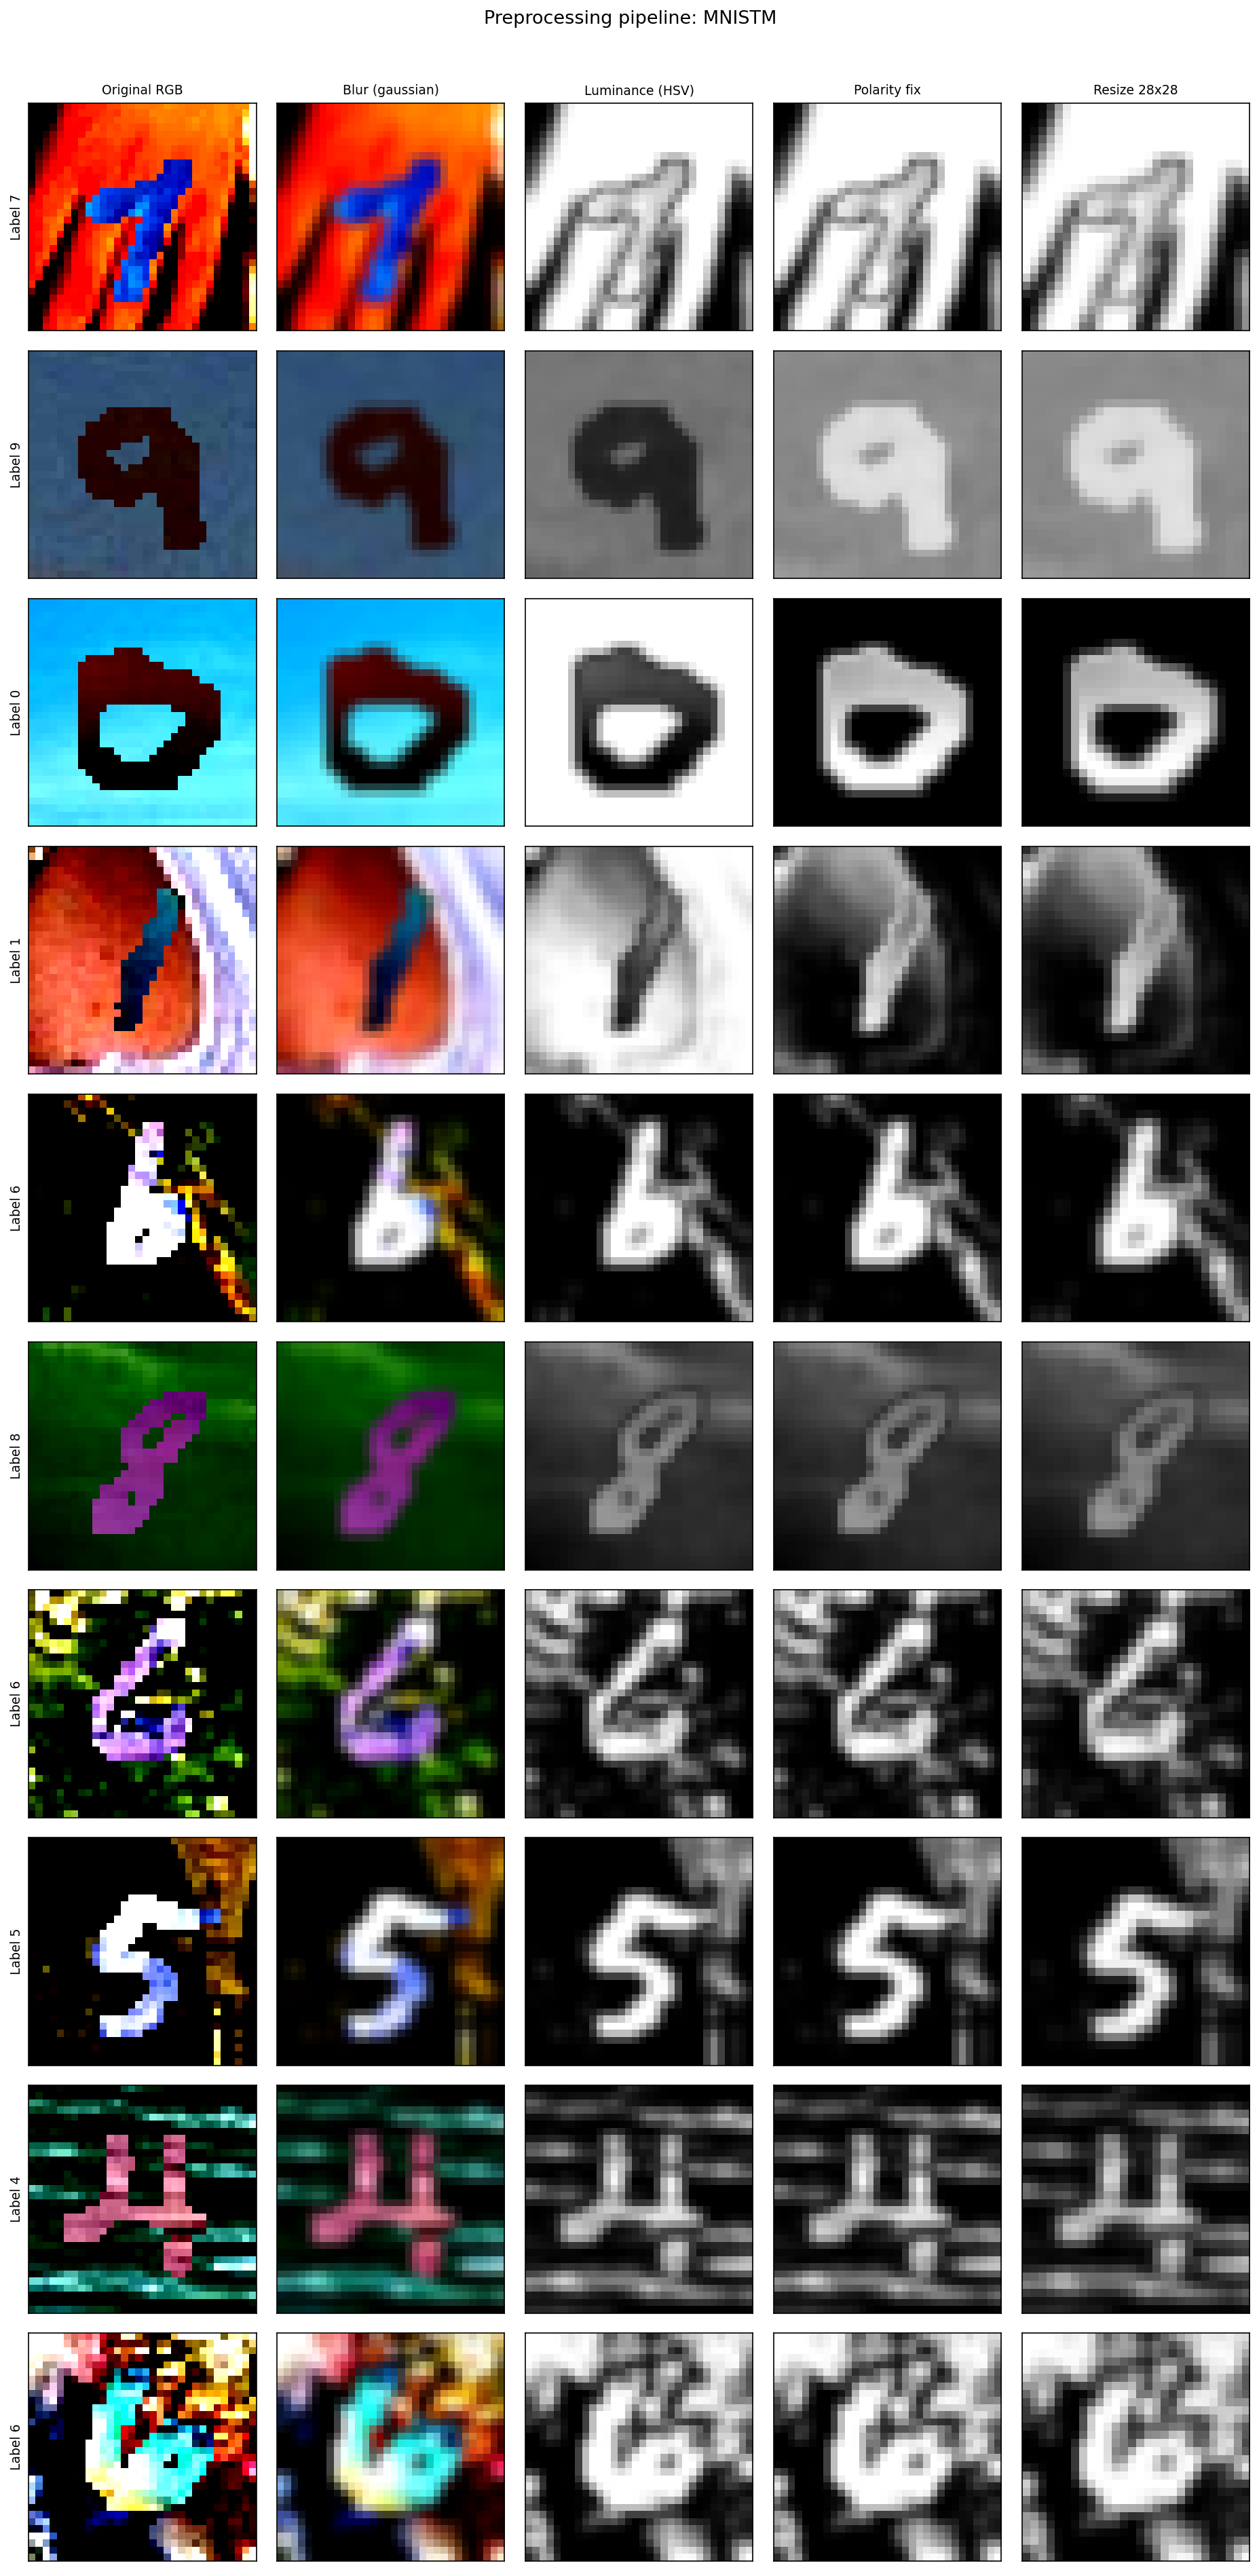
\includegraphics[width=\linewidth,height=0.82\textheight,keepaspectratio]{checkpoints/pipeline_mnistm.png}
        \caption{MNIST-M: imagen original RGB $\rightarrow$ escala de grises (\textit{luminance}) $\rightarrow$ \textit{blur} gaussiano $\rightarrow$ corrección de polaridad $\rightarrow$ \textit{resize} a $28\times28$.}
        \label{fig:pipeline_mnistm}
    \end{subfigure}
    \hfill
    \begin{subfigure}[t]{0.53\linewidth}
        \centering
        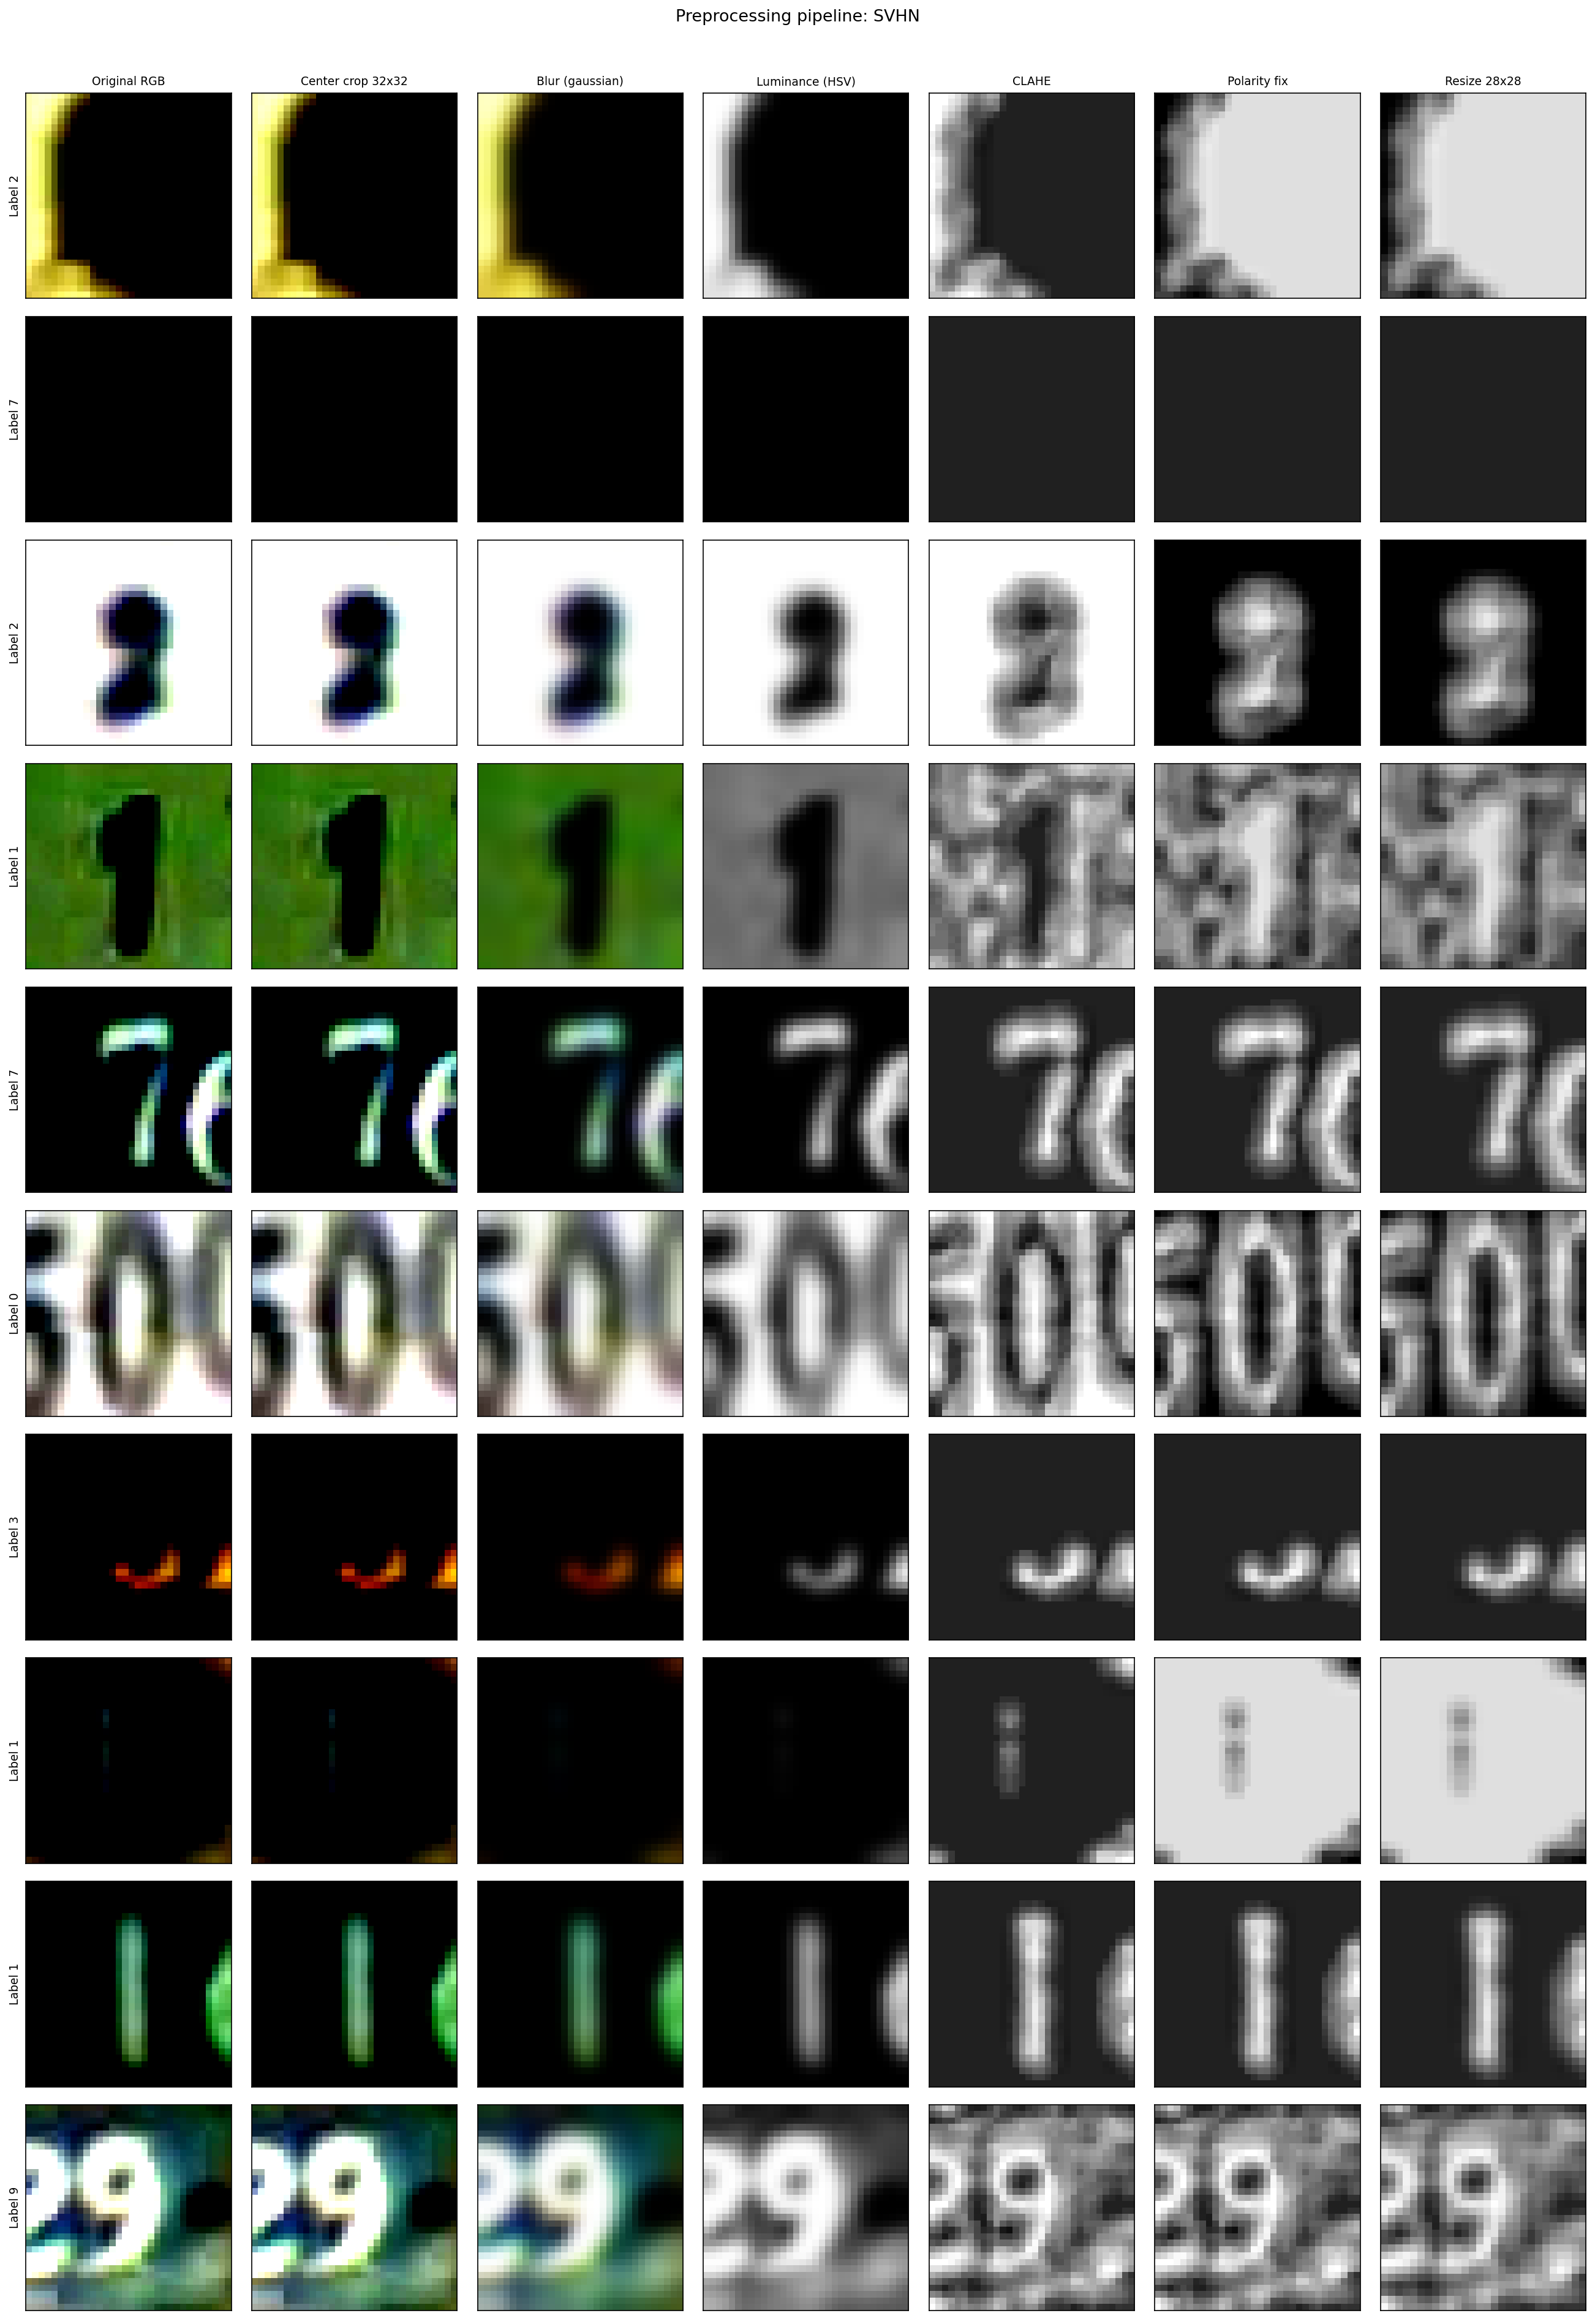
\includegraphics[width=\linewidth,height=0.82\textheight,keepaspectratio]{checkpoints/pipeline_svhn.png}
        \caption{SVHN: idéntico al pipeline de MNIST-M, con un \textit{center crop} inicial para descartar dígitos vecinos.}
        \label{fig:pipeline_svhn}
    \end{subfigure}
    \caption{Pipeline de preprocesamiento aplicado a imágenes de MNIST-M (izquierda) y SVHN (derecha). Cada fila de cada panel muestra una imagen pasando por las etapas sucesivas del pipeline.}
    \label{fig:pipelines}
\end{figure}

\section{DANN}

Domain Adversarial Neural Networks (DANN) es un método diseñado específicamente para el cambio de dominio. En estos problemas, se tiene datos etiquetados en un dominio, y datos no etiquetados en otro dominio. En nuestro caso, trabajamos con MNIST como datos etiquetados y MNIST-M como datos no etiquetados. El objetivo es lograr que el modelo pueda clasificar datos de MNIST-M (y también MNIST) a pesar de no tener etiquetas de los datos de MNIST-M.

DANN tiene tres módulos entrenables para alcanzar este objetivo: un encoder y dos clasificadores. Uno de los clasificadores devuelve la clase del dato de entrada, y el otro devuelve el dominio de la clase. Sin embargo, el encoder y el clasificador de dominios trabajan adversarialmente. El encoder intentará de lograr representaciones invariantes al dominio para confundir al clasificador de dominios, mientras que este intentará clasificar el dominio a partir de las representaciones lo mejor que pueda. El resultado final es un encoder que logra representaciones muy similares de los datos para ambos dominios. Una vez terminado el entrenamiento, se descarta el clasificador de dominios y se utiliza solamente el encoder y el otro clasificador.

Para entrenar una DANN, en cada batch se forman dos forwards. En el primero se pasan imágenes de MNIST con etiquetas para calcular la pérdida de clasificación $\mathcal{L}_{cls}$ y, sobre los mismos features, se pasa también por el clasificador de dominios para calcular la parte source de la pérdida de dominio. En el segundo se pasan imágenes de MNIST-M sin etiquetas, únicamente para alimentar al clasificador de dominios y completar $\mathcal{L}_{dom}$. La pérdida total es entonces

\begin{equation}
    \mathcal{L} = \mathcal{L}_{cls}(\text{MNIST}) - \lambda \cdot \mathcal{L}_{dom}(\text{MNIST + MNIST-M})
\end{equation}

donde el signo negativo lo introduce la GRL automáticamente en el \textit{backward pass}. El coeficiente $\lambda$ no es constante, sino que sigue el \textit{schedule} propuesto por Ganin et al.,

\begin{equation}
    \lambda_p = \frac{2}{1 + \exp(-10\,p)} - 1, \qquad p \in [0, 1]
\end{equation}

con $p$ el progreso normalizado del entrenamiento. La idea es que al principio, cuando los features todavía no son informativos, la presión adversarial sea pequeña para que el encoder aprenda primero a clasificar y recién después intente alinear dominios. Si $\lambda$ arranca demasiado grande, los gradientes invertidos terminan haciendo explotar el encoder, algo que verificamos en la práctica.

En cuanto a la implementación, mantuvimos el encoder idéntico al de las partes anteriores (\textit{ConvNetEncoder} de cuatro bloques, hidden\_dim = 64). Las dos cabezas son redes FC pequeñas: una capa lineal de 64 a 512, ReLU, y otra capa lineal de 512 a la cantidad de clases (10 para la cabeza de tarea, 2 para la de dominio). Una decisión importante fue cómo pasarle las imágenes al modelo. La consigna sugiere usar la misma arquitectura que en las partes anteriores ``para facilitar la comparación'', y en un primer momento intentamos también usar el mismo pipeline de preprocesamiento (las imágenes de MNIST-M reducidas a escala de grises). Pero esto resultó catastrófico: el discriminador de dominios alcanzaba 100\% de accuracy en una sola época y la GRL hacía explotar al encoder. La razón es que las estadísticas de entrada de MNIST (normalizado con su media y desvío) y de MNIST-M (en $[0,1]$ luego del preprocesamiento) son muy distintas, y el discriminador puede separarlos trivialmente sin mirar los dígitos. Resolvimos esto pasando ambos dominios como imágenes RGB de tres canales con la misma normalización $\mathcal{N}(0.5, 0.5)$. Con eso el discriminador se ve forzado a mirar features semánticos y el entrenamiento se vuelve estable. Es la única desviación respecto al pipeline de las partes anteriores, y la \textit{justificamos} porque para DANN es estrictamente necesaria.

El optimizador fue Adam con \textit{learning rate} $10^{-3}$ y \textit{weight decay} $10^{-4}$. Sumamos \textit{gradient clipping} con norma máxima 1.0 antes de cada paso del optimizador. El \textit{weight decay} es importante para frenar el sobreajuste del encoder a MNIST: sin él, $\mathcal{L}_{cls}$ baja a casi cero muy rápido y luego el gradiente sigue tirando los features hacia características específicas del dominio fuente, lo cual deteriora lentamente la accuracy en MNIST-M. El \textit{clipping} es el truco estándar para estabilizar entrenamientos adversariales: cuando el discriminador gana por mucho en alguna época temprana, la GRL puede inyectar un gradiente enorme que descontrola al encoder; acotando la norma garantizamos que ningún paso pueda romper el equilibrio del juego adversarial.

Entrenamos por 60 épocas con \textit{batch size} 64. Además, entrenamos en paralelo un \textit{baseline} idéntico pero sin GRL ni $\mathcal{L}_{dom}$, simplemente un clasificador entrenado sobre MNIST, para tener una referencia clara de cuánto aporta la adaptación de dominio. La Tabla~\ref{tab:hp_dann} resume los hiperparámetros utilizados.

\begin{table}[h]
    \centering
    \begin{tabular}{ll}
        \hline
        Hiperparámetro                          & Valor                       \\
        \hline
        Épocas                                  & 60                          \\
        \textit{Batch size}                     & 64                          \\
        Optimizador                             & Adam                        \\
        \textit{Learning rate}                  & $10^{-3}$                   \\
        \textit{Weight decay}                   & $10^{-4}$                   \\
        \textit{Gradient clipping} (norma máx.) & 1.0                         \\
        Encoder                                 & ConvNetEncoder (4 bloques)  \\
        Dimensión del \textit{embedding} (\textit{hidden\_dim}) & 64          \\
        Cabezas $G_y$ y $G_d$ (\textit{head\_dim})              & 512         \\
        Entrada (\textit{input\_mode})          & RGB 3 canales, \textit{Normalize}(0.5, 0.5) \\
        \textit{Schedule} de $\lambda$          & $\lambda_p = 2/(1+e^{-10p}) - 1$ \\
        \textit{Seed}                           & 42                          \\
        \hline
    \end{tabular}
    \caption{Hiperparámetros utilizados para entrenar DANN sobre MNIST $\rightarrow$ MNIST-M. El \textit{baseline} usa la misma configuración pero sin GRL ni $\mathcal{L}_{dom}$.}
    \label{tab:hp_dann}
\end{table}

A diferencia de los métodos anteriores, para DANN sí corrimos un \textit{grid search} estructurado y guardamos los resultados de cada combinación. La Tabla~\ref{tab:gs_dann} muestra el espacio explorado: tres \textit{learning rates} (con dos configuraciones de \textit{schedule}), tres anchos de encoder, dos anchos de cabeza y dos tamaños de \textit{batch}, lo cual da un total de \textbf{36 configuraciones}.

\begin{table}[H]
    \centering
    \begin{tabular}{ll}
        \hline
        Hiperparámetro                       & Valores explorados \\
        \hline
        \textit{Learning rate}               & $\{10^{-3},\, 2\cdot 10^{-3},\, 5\cdot 10^{-3}\}$ \\
        \textit{LR schedule} de Ganin $\mu_p = \mu_0/(1+10p)^{0.75}$ & $\{\text{off},\, \text{on}\}$ \\
        \textit{hidden\_dim} (ancho del encoder) & $\{128,\, 192,\, 256\}$ \\
        \textit{head\_dim} (ancho de las cabezas $G_y$, $G_d$) & $\{256,\, 512\}$ \\
        \textit{Batch size}                  & $\{128,\, 256\}$ \\
        Épocas                               & 40 (fijo) \\
        \textit{Weight decay}                & $10^{-5}$ (fijo) \\
        \textit{Subset} de MNIST / MNIST-M   & $20\,000$ imágenes c/u (fijo) \\
        \hline
    \end{tabular}
    \caption{Espacio de búsqueda del \textit{grid search} de DANN: $3 \times 2 \times 3 \times 2 \times 2 = 36$ configuraciones, evaluadas sobre un \textit{split} de validación de MNIST-M de 5\,000 imágenes.}
    \label{tab:gs_dann}
\end{table}

La Tabla~\ref{tab:gs_dann_top5} reporta las cinco mejores configuraciones del barrido ordenadas por la mejor accuracy alcanzada en la validación de MNIST-M durante el entrenamiento. La configuración ganadora coincide en estructura con la que usamos para el entrenamiento final de la Tabla~\ref{tab:hp_dann}: \textit{learning rate} $10^{-3}$, \textit{schedule} apagado, \textit{head\_dim} $512$ y \textit{batch size} pequeño (entre los explorados). Para el entrenamiento final escalamos a 60 épocas y agregamos \textit{weight decay} $10^{-4}$ y \textit{gradient clipping}, lo cual nos permitió mantener un \textit{batch size} de 64 y obtener resultados más altos en \textit{test} que los reportados acá.

\begin{table}[H]
    \centering
    \begin{tabular}{lcccccc}
        \hline
        \# & lr & \textit{schedule} & hidden & head & bs & best tgt acc \\
        \hline
        1 & $10^{-3}$     & off & 256 & 512 & 128 & 71.44\% \\
        2 & $10^{-3}$     & off & 192 & 512 & 128 & 70.82\% \\
        3 & $10^{-3}$     & off & 128 & 512 & 128 & 70.64\% \\
        4 & $2\cdot 10^{-3}$ & off & 128 & 512 & 128 & 70.46\% \\
        5 & $2\cdot 10^{-3}$ & off & 192 & 512 & 128 & 70.28\% \\
        \hline
    \end{tabular}
    \caption{Top 5 configuraciones del \textit{grid search} de DANN, ordenadas por la mejor accuracy de validación sobre MNIST-M durante el entrenamiento. Las 36 configuraciones completas están en \texttt{checkpoints/gridsearch\_dann.csv}.}
    \label{tab:gs_dann_top5}
\end{table}

\section{Resultados}

Las accuracies \textit{cross-domain} reportadas en 4.1.3 y 4.2.4 se midieron con la misma configuración para los tres modelos: episodios 10-way, $Q=10$, 200 episodios por celda y $K \in \{1, 2, 4, 8, 16\}$.

\subsection{4.1.2 — Entrenamiento y análisis \textit{in-domain} (ProtoNets)}

ProtoNet alcanzó $98.40\%$ de accuracy de query en validación en la época 16 (Figura~\ref{fig:val_query_acc_protonet}). La accuracy de support coincide con la de query, indicando que el espacio latente generaliza dentro del episodio en vez de memorizar. La proyección t-SNE \textit{in-domain} de la Figura~\ref{fig:tsne_protonet_indomain} muestra los diez dígitos en \textit{clusters} bien separados, como espera la pérdida basada en distancia a prototipos.

\begin{figure}[h]
    \centering
    \begin{subfigure}[t]{0.49\linewidth}
        \centering
        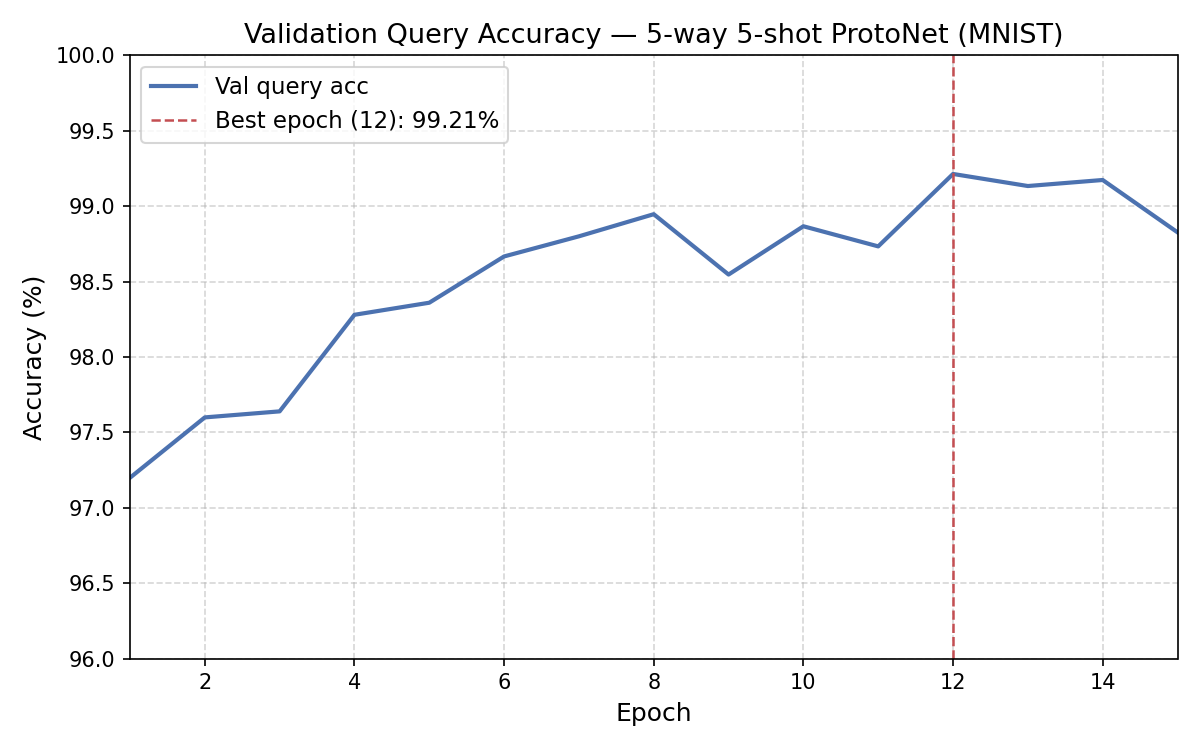
\includegraphics[width=\linewidth]{checkpoints/val_query_acc.png}
        \caption{Accuracy de query en validación.}
        \label{fig:val_query_acc_protonet}
    \end{subfigure}
    \hfill
    \begin{subfigure}[t]{0.49\linewidth}
        \centering
        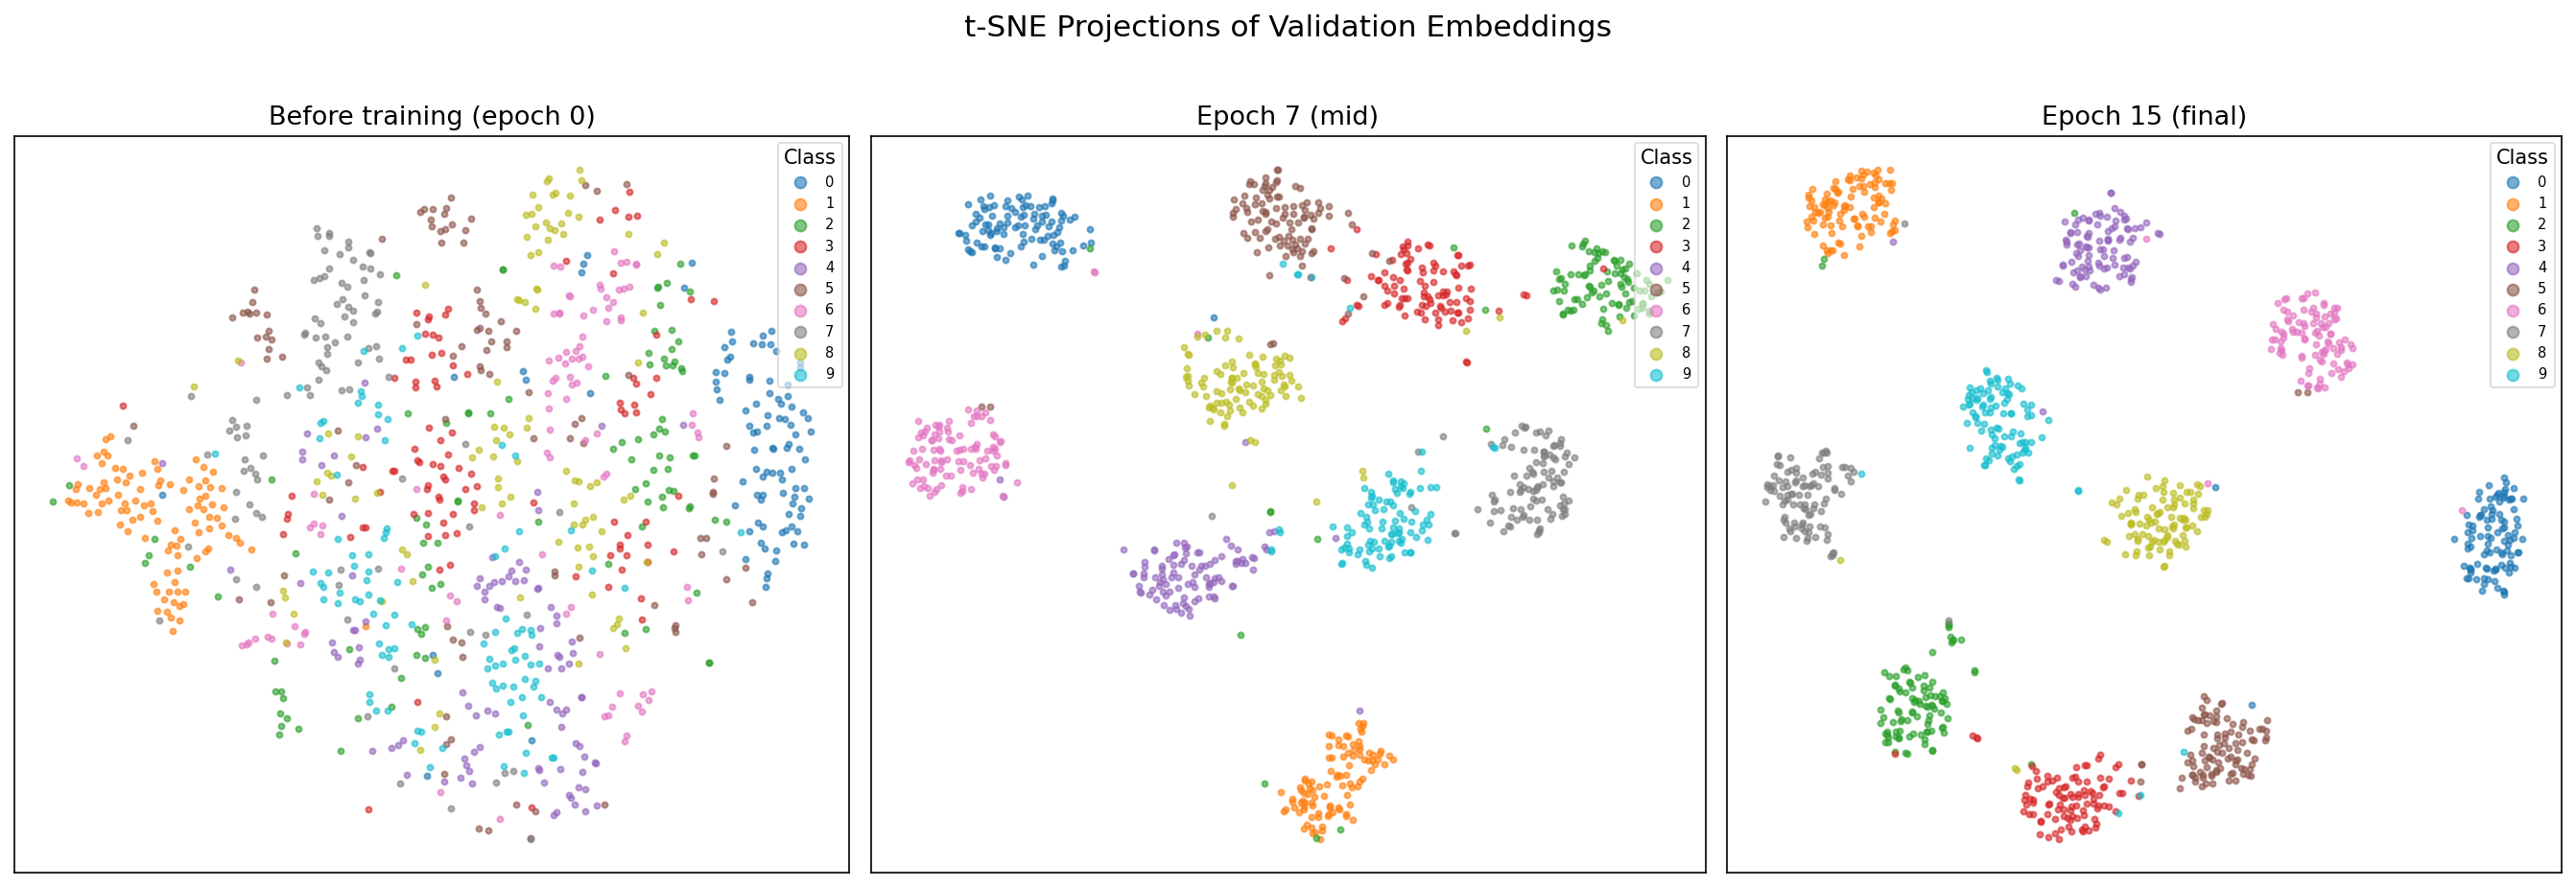
\includegraphics[width=\linewidth]{checkpoints/tsne_embeddings.png}
        \caption{t-SNE \textit{in-domain} sobre MNIST.}
        \label{fig:tsne_protonet_indomain}
    \end{subfigure}
    \caption{ProtoNet entrenado sobre MNIST: curva de validación (izquierda) y proyección t-SNE de \textit{embeddings} coloreados por clase (derecha).}
\end{figure}

\subsection{4.1.3 — Evaluación \textit{cross-domain} (ProtoNets)}

La Figura~\ref{fig:cross_domain_protonet} grafica la accuracy de ProtoNet en función de $K$ para los tres dominios. Los valores numéricos se reportan junto con el resto de modelos en la Tabla~\ref{tab:comparison} de la subsección 4.2.4. La Figura~\ref{fig:embedding_scatter} muestra el t-SNE \textit{cross-domain}: MNIST y MNIST-M ocupan regiones disjuntas del espacio latente, lo cual explica geométricamente la brecha de accuracy (un prototipo armado con muestras de MNIST queda lejos de queries del mismo dígito en MNIST-M).

\begin{figure}[h]
    \centering
    \begin{subfigure}[t]{0.55\linewidth}
        \centering
        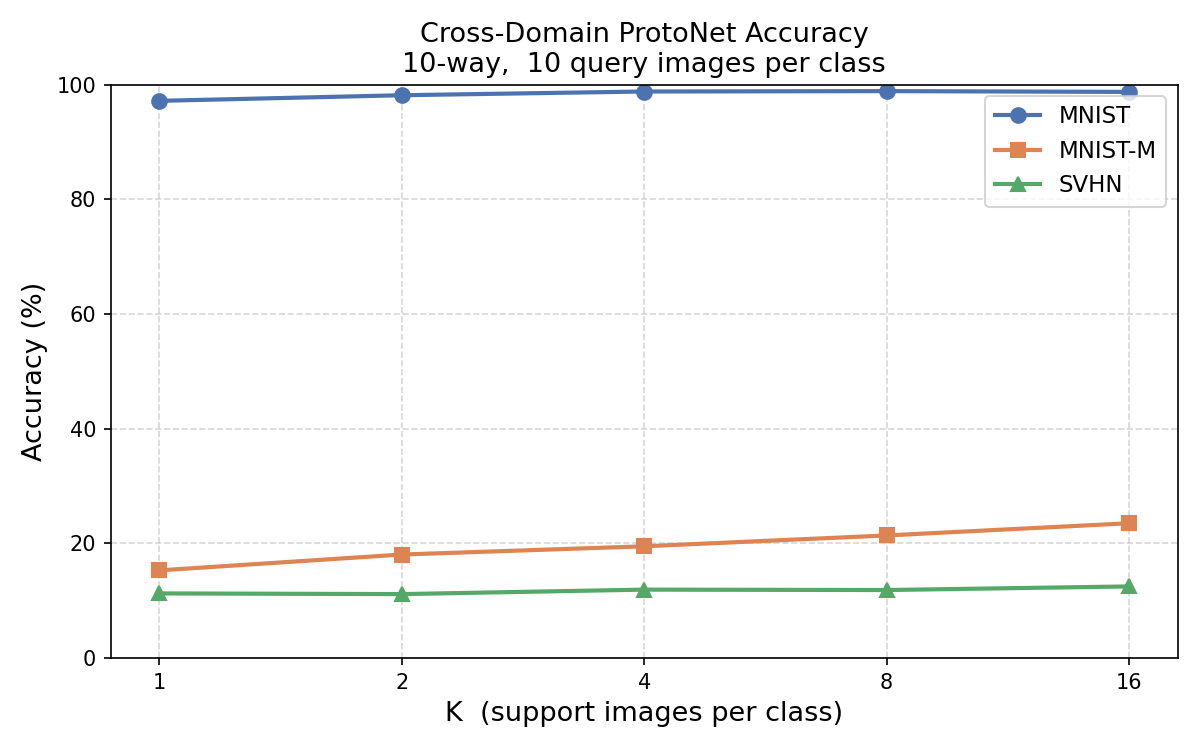
\includegraphics[width=\linewidth]{checkpoints/cross_domain_accuracy.png}
        \caption{Accuracy vs $K$ para ProtoNet en los tres dominios.}
        \label{fig:cross_domain_protonet}
    \end{subfigure}
    \hfill
    \begin{subfigure}[t]{0.42\linewidth}
        \centering
        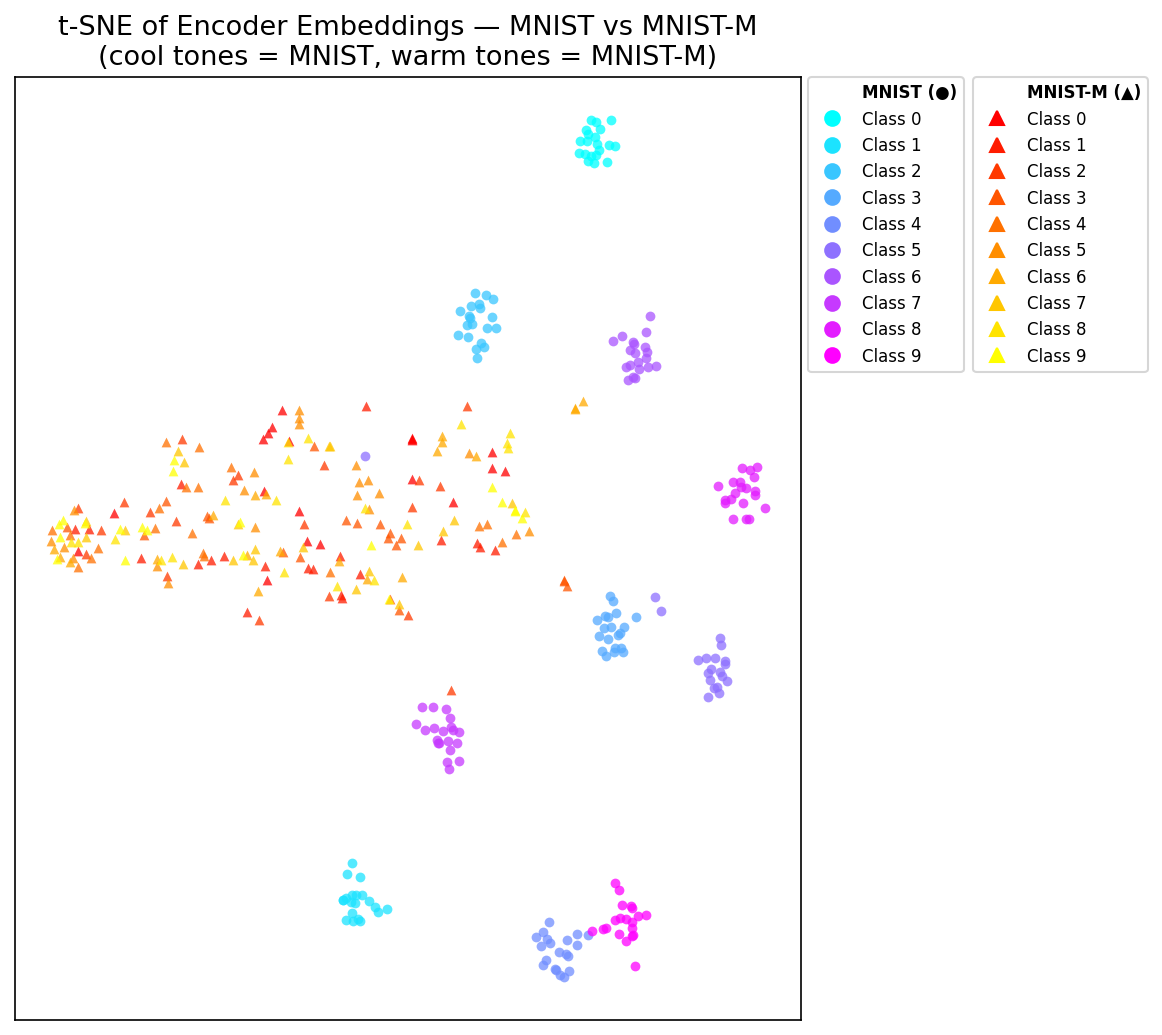
\includegraphics[width=\linewidth]{checkpoints/embedding_scatter.png}
        \caption{t-SNE de MNIST y MNIST-M con el encoder de ProtoNet.}
        \label{fig:embedding_scatter}
    \end{subfigure}
    \caption{ProtoNet en evaluación \textit{cross-domain}: accuracy vs $K$ y proyección t-SNE coloreada por dominio y por clase.}
\end{figure}

\subsection{4.2.2 — Implementación de MAML}

MAML alcanzó $97.57\%$ de accuracy de query post-adaptación en validación (mejor época: 43). ProtoMAML alcanzó $97.41\%$ en la época 36 con una curva más suave y convergencia más temprana, lo cual es coherente con que la inicialización por prototipos provee un punto de partida semánticamente significativo. Las dos curvas se ven en la Figura~\ref{fig:val_query_maml_protomaml}.

\begin{figure}[h]
    \centering
    \begin{subfigure}[t]{0.49\linewidth}
        \centering
        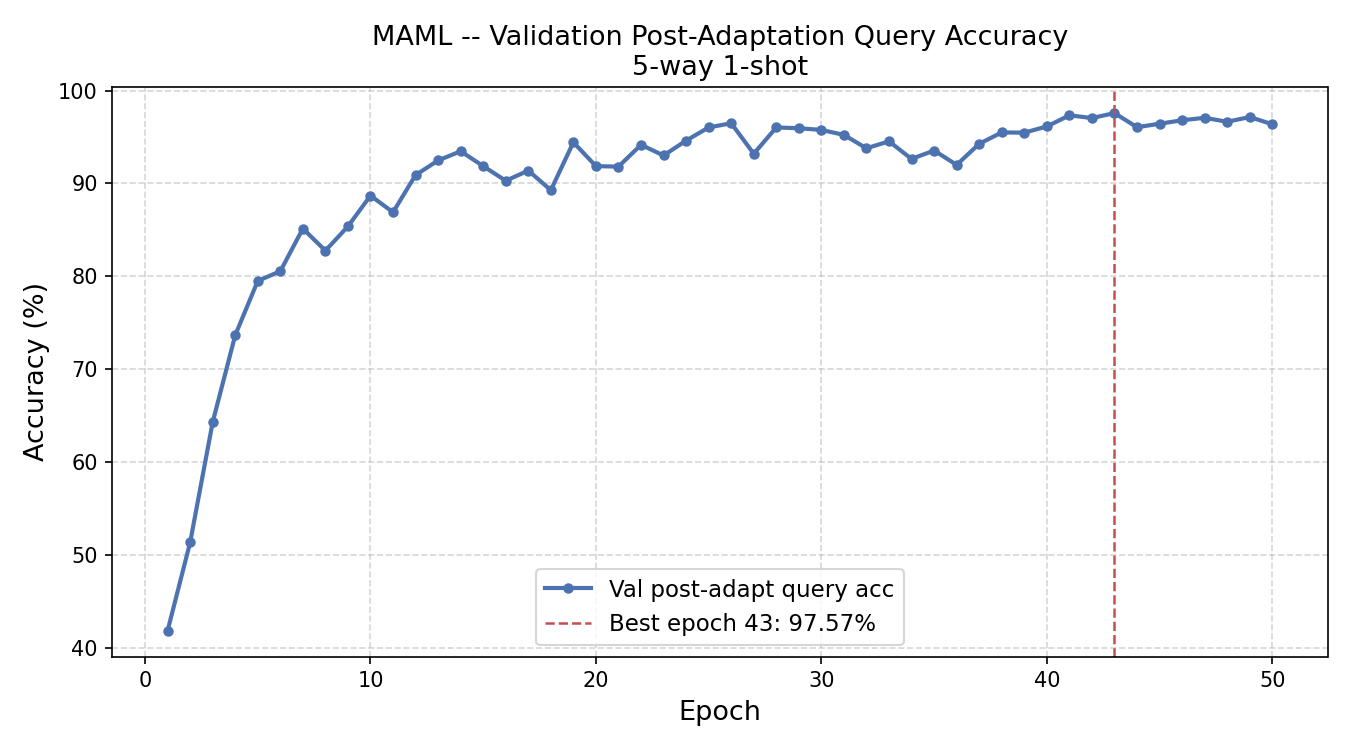
\includegraphics[width=\linewidth]{checkpoints/val_query_acc_best_maml.png}
        \caption{MAML.}
        \label{fig:val_query_acc_maml}
    \end{subfigure}
    \hfill
    \begin{subfigure}[t]{0.49\linewidth}
        \centering
        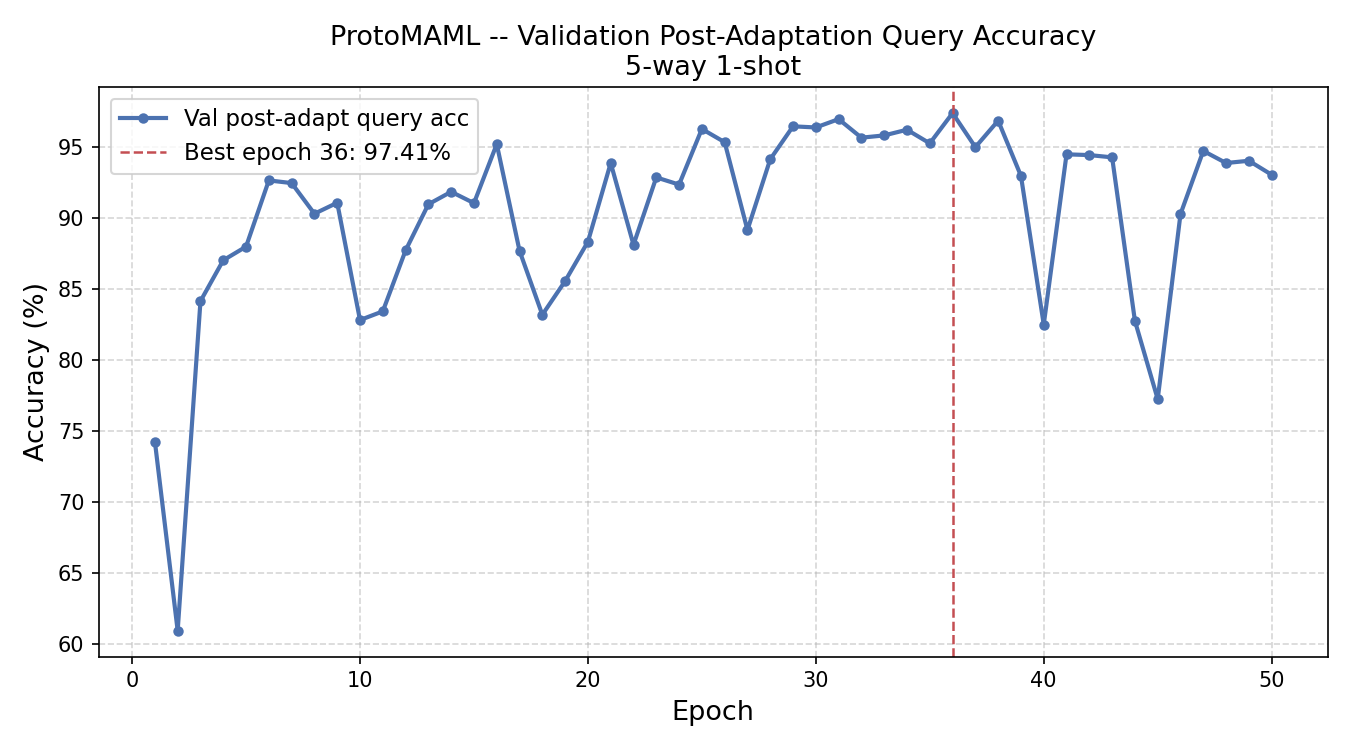
\includegraphics[width=\linewidth]{checkpoints/val_query_acc_best_protomaml.png}
        \caption{ProtoMAML.}
        \label{fig:val_query_acc_protomaml}
    \end{subfigure}
    \caption{Accuracy de query post-adaptación en validación (5-way 1-shot, $Q=15$).}
    \label{fig:val_query_maml_protomaml}
\end{figure}

\subsection{4.2.4 — Comparación final: ProtoNet vs MAML vs ProtoMAML}

La Tabla~\ref{tab:comparison} reporta las accuracies para los tres modelos en los tres dominios. La Figura~\ref{fig:comparison} las grafica.

\begin{table}[h]
    \centering
    \begin{tabular}{llccccc}
        \hline
        Dominio                  & Modelo     & $K=1$  & $K=2$  & $K=4$  & $K=8$  & $K=16$ \\
        \hline
        \multirow{3}{*}{MNIST}   & ProtoNet   & 91.5\% & 95.1\% & 96.4\% & 96.8\% & 96.8\% \\
                                 & MAML       & 83.1\% & 89.2\% & 91.3\% & 93.3\% & 93.1\% \\
                                 & ProtoMAML  & \textbf{95.8\%} & \textbf{96.8\%} & \textbf{97.1\%} & \textbf{97.3\%} & \textbf{97.1\%} \\
        \hline
        \multirow{3}{*}{MNIST-M} & ProtoNet   & 33.0\% & 39.1\% & 45.9\% & 51.4\% & 55.3\% \\
                                 & MAML       & 17.4\% & 15.8\% & 15.8\% & 15.5\% & 14.4\% \\
                                 & ProtoMAML  & \textbf{42.0\%} & \textbf{52.3\%} & \textbf{59.4\%} & \textbf{62.3\%} & \textbf{64.6\%} \\
        \hline
        \multirow{3}{*}{SVHN}    & ProtoNet   & \textbf{16.4\%} & 18.2\% & 21.4\% & 24.4\% & 27.3\% \\
                                 & MAML       & 10.9\% & 11.2\% & 10.7\% & 10.9\% & 10.7\% \\
                                 & ProtoMAML  & \textbf{16.4\%} & \textbf{19.0\%} & \textbf{23.2\%} & \textbf{26.4\%} & \textbf{28.4\%} \\
        \hline
    \end{tabular}
    \caption{Accuracy episódica \textit{cross-domain} (10-way, $Q=10$, 200 episodios). El mejor modelo por celda se indica en negrita.}
    \label{tab:comparison}
\end{table}

\begin{figure}[h]
    \centering
    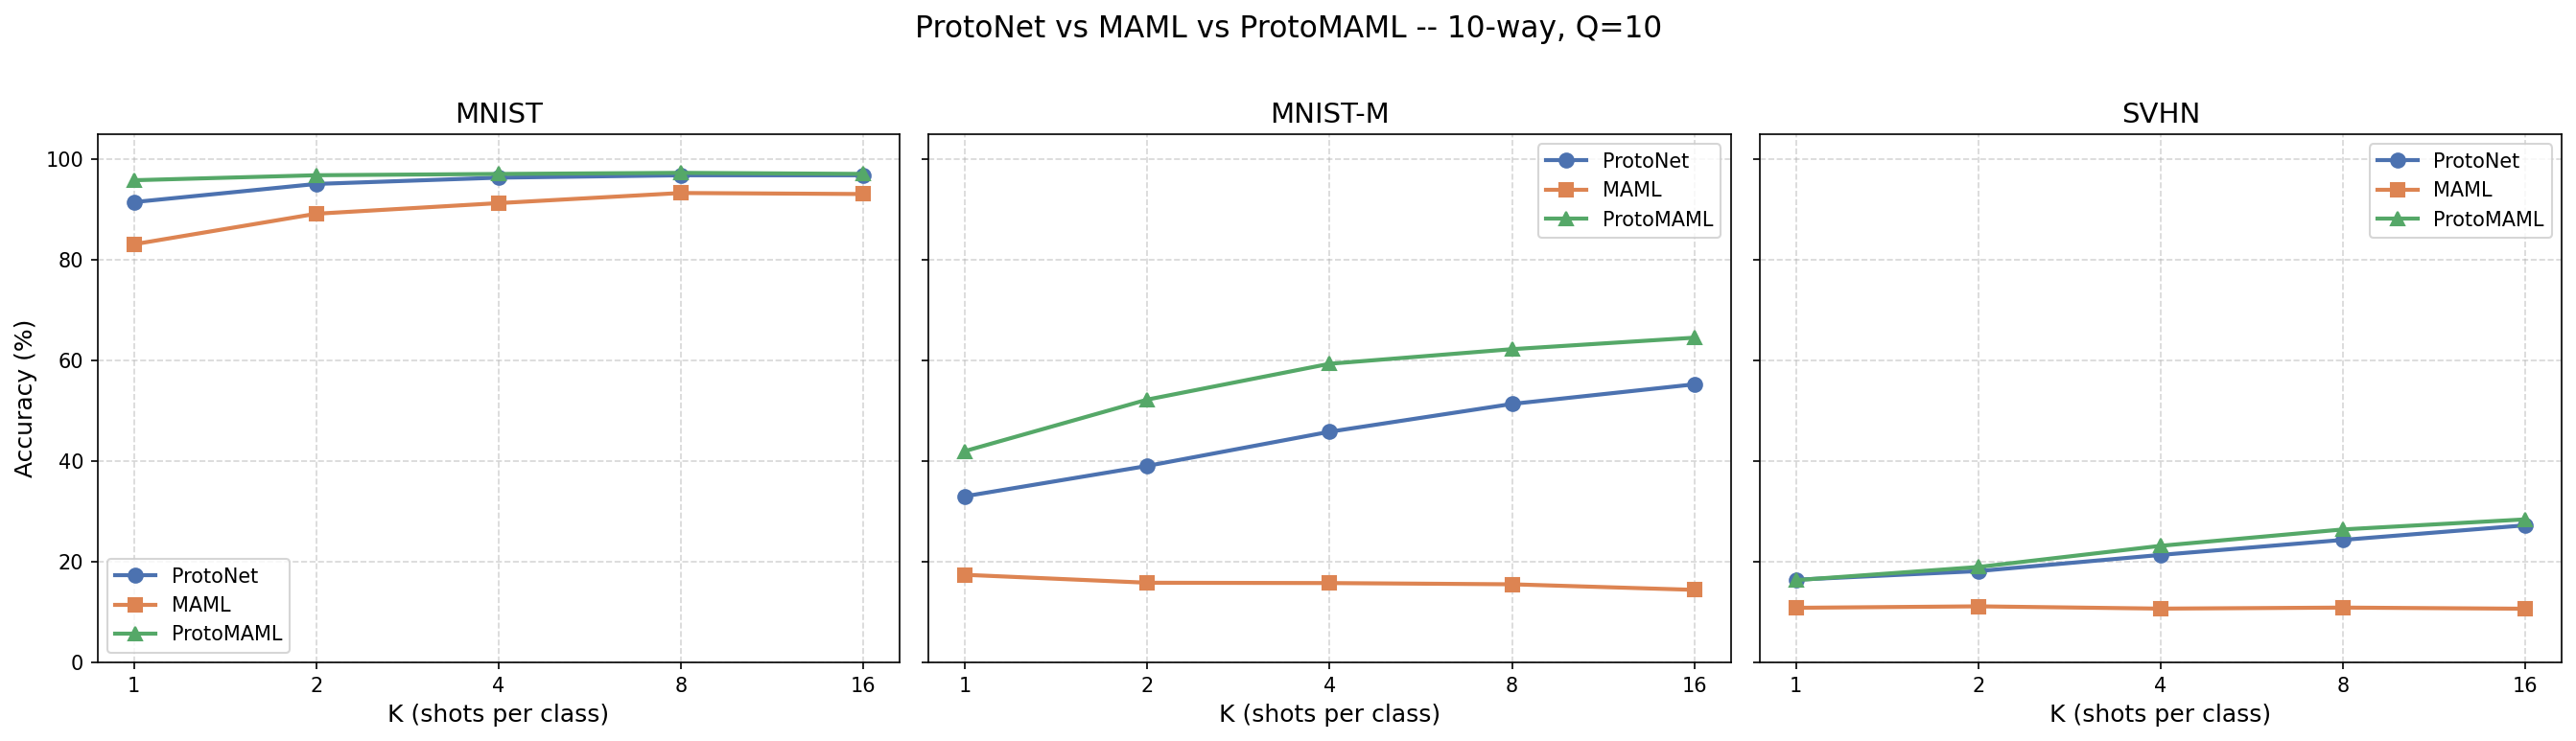
\includegraphics[width=\linewidth]{checkpoints/comparison_protonet_maml_protomaml.png}
    \caption{Accuracy \textit{cross-domain} vs $K$ para los tres modelos en los tres dominios.}
    \label{fig:comparison}
\end{figure}

Tres observaciones del cuadro. ProtoMAML domina casi todas las celdas; su ventaja se hace notable en MNIST-M ($64.6\%$ vs $55.3\%$ de ProtoNet con $K=16$). MAML puro colapsa en \textit{cross-domain}: $\sim 15\%$ en MNIST-M sin mejorar con $K$ y $\sim 11\%$ en SVHN (azar en 10-way). En SVHN ningún método supera el $28\%$, lo cual señala que la brecha de dominio con MNIST es demasiado grande para cerrarse vía \textit{meta-learning} solo. La Figura~\ref{fig:tsne_all_models} confirma esto: en los tres encoders, los dominios siguen separados en el espacio latente. Esta limitación motiva la Parte 4.

\begin{figure}[h]
    \centering
    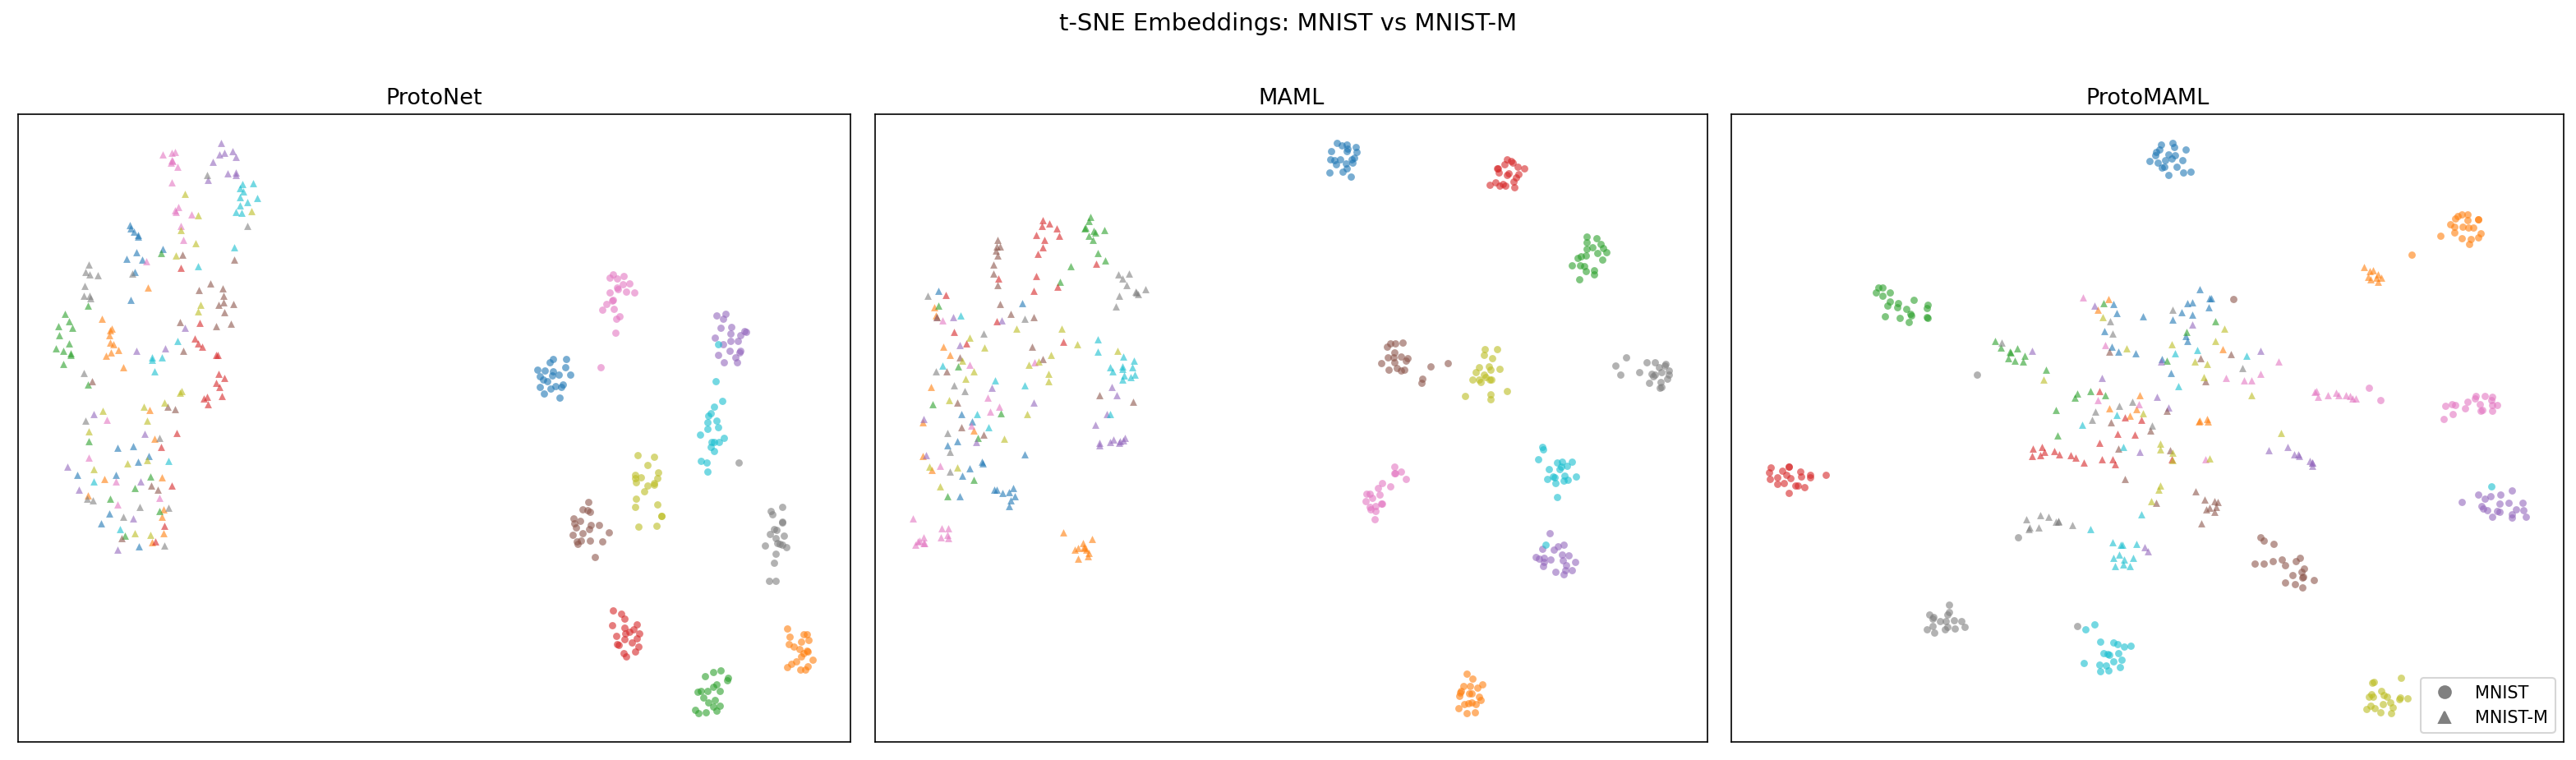
\includegraphics[width=\linewidth]{checkpoints/tsne_comparison_all_models.png}
    \caption{t-SNE de \textit{embeddings} de MNIST, MNIST-M y SVHN con los encoders de los tres modelos, coloreados por dominio.}
    \label{fig:tsne_all_models}
\end{figure}

\subsection{4.3.2 — Análisis de resultados (DANN)}

La Figura~\ref{fig:dann_curves} muestra las tres curvas pedidas. La $\mathcal{L}_{dom}$ de DANN sube de $0.37$ y se estabiliza cerca de $\ln(2) \approx 0.693$, y la \textit{domain accuracy} cae de $88\%$ a $\sim 54\%$: el encoder logró representaciones que el discriminador no puede separar por dominio. En MNIST-M, el \textit{baseline} pica cerca del $57\%$ y luego decae (sobreajuste al \textit{source}), mientras que DANN sube sostenidamente y se estabiliza entre $71\%$ y $74\%$ gracias al \textit{weight decay} que frena la deriva post-pico.

\begin{figure}[h]
    \centering
    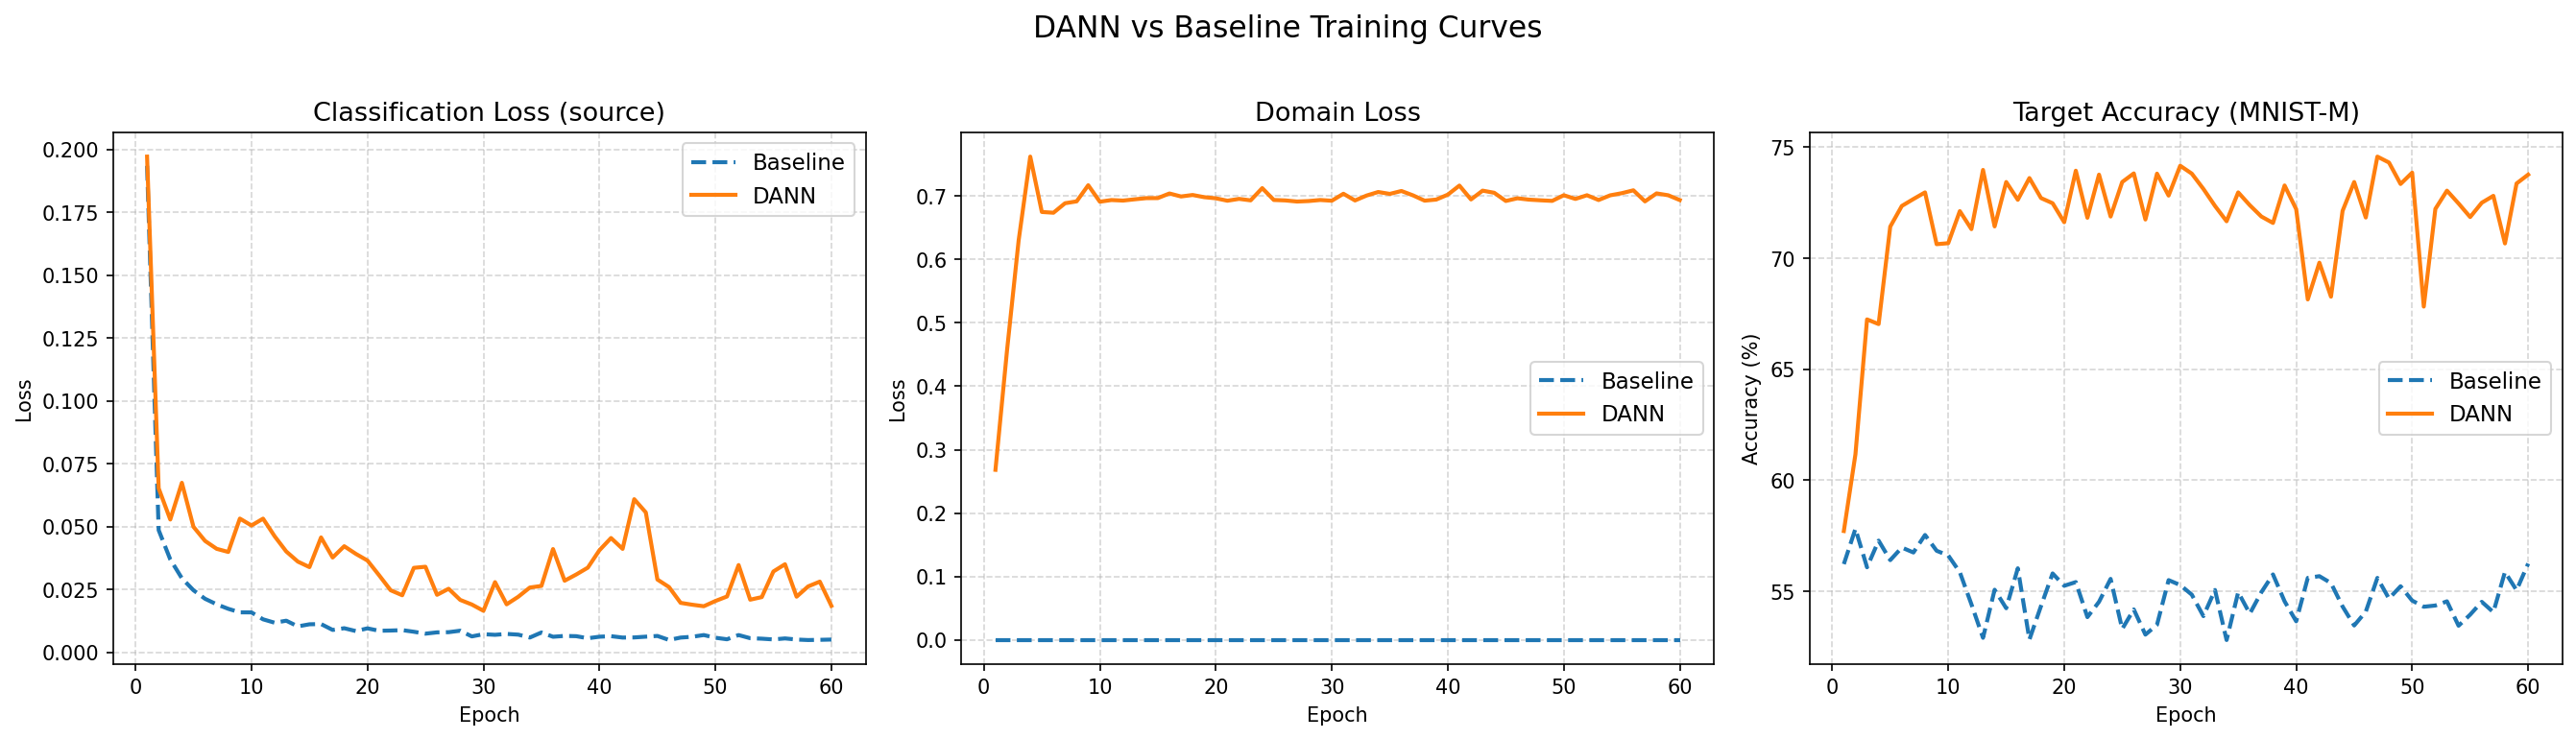
\includegraphics[width=\linewidth]{checkpoints/dann_training_curves.png}
    \caption{Curvas de entrenamiento de DANN vs \textit{baseline}: $\mathcal{L}_{cls}$, $\mathcal{L}_{dom}$ y accuracy en MNIST-M.}
    \label{fig:dann_curves}
\end{figure}

\begin{table}[h]
    \centering
    \begin{tabular}{lcc}
        \hline
        Modelo   & Source (MNIST) & Target (MNIST-M) \\
        \hline
        Baseline & 99.11\%        & 56.25\%          \\
        DANN     & 99.09\%        & \textbf{73.77\%} \\
        \hline
    \end{tabular}
    \caption{Accuracy final en \textit{source} y \textit{target} (test sets, última época).}
    \label{tab:dann_results}
\end{table}

DANN obtiene \textbf{$+17.5$ puntos} sobre el \textit{baseline} en MNIST-M sin haber usado ninguna etiqueta del dominio target, y sin degradar la accuracy en \textit{source} ($99.09\%$ vs $99.11\%$). Notablemente, esos $73.77\%$ superan también al mejor método de \textit{meta-learning} sobre MNIST-M ($64.6\%$ de ProtoMAML con $K=16$): exponer al modelo a datos no etiquetados del \textit{target} durante el entrenamiento es más efectivo que adaptar con $K$ muestras etiquetadas en \textit{test time}.

\subsection{4.3.3 — Visualización del espacio latente: antes y después de la adaptación}

La Figura~\ref{fig:dann_tsne} compara el espacio latente en tres momentos. \textit{Por dominio} (fila superior), MNIST y MNIST-M están claramente separados en el encoder preentrenado y en el \textit{baseline}, y se entremezclan en DANN — la contraparte cualitativa del $54\%$ de \textit{domain accuracy} final. \textit{Por clase} (fila inferior), los \textit{clusters} del preentrenado y del \textit{baseline} contienen puntos de un solo dominio; en DANN los \textit{clusters} agrupan ambos dominios por dígito, mostrando que el encoder produce representaciones invariantes al dominio. Esa propiedad es la explicación geométrica de los $17.5$ puntos de mejora en la Tabla~\ref{tab:dann_results}.

\begin{figure}[h]
    \centering
    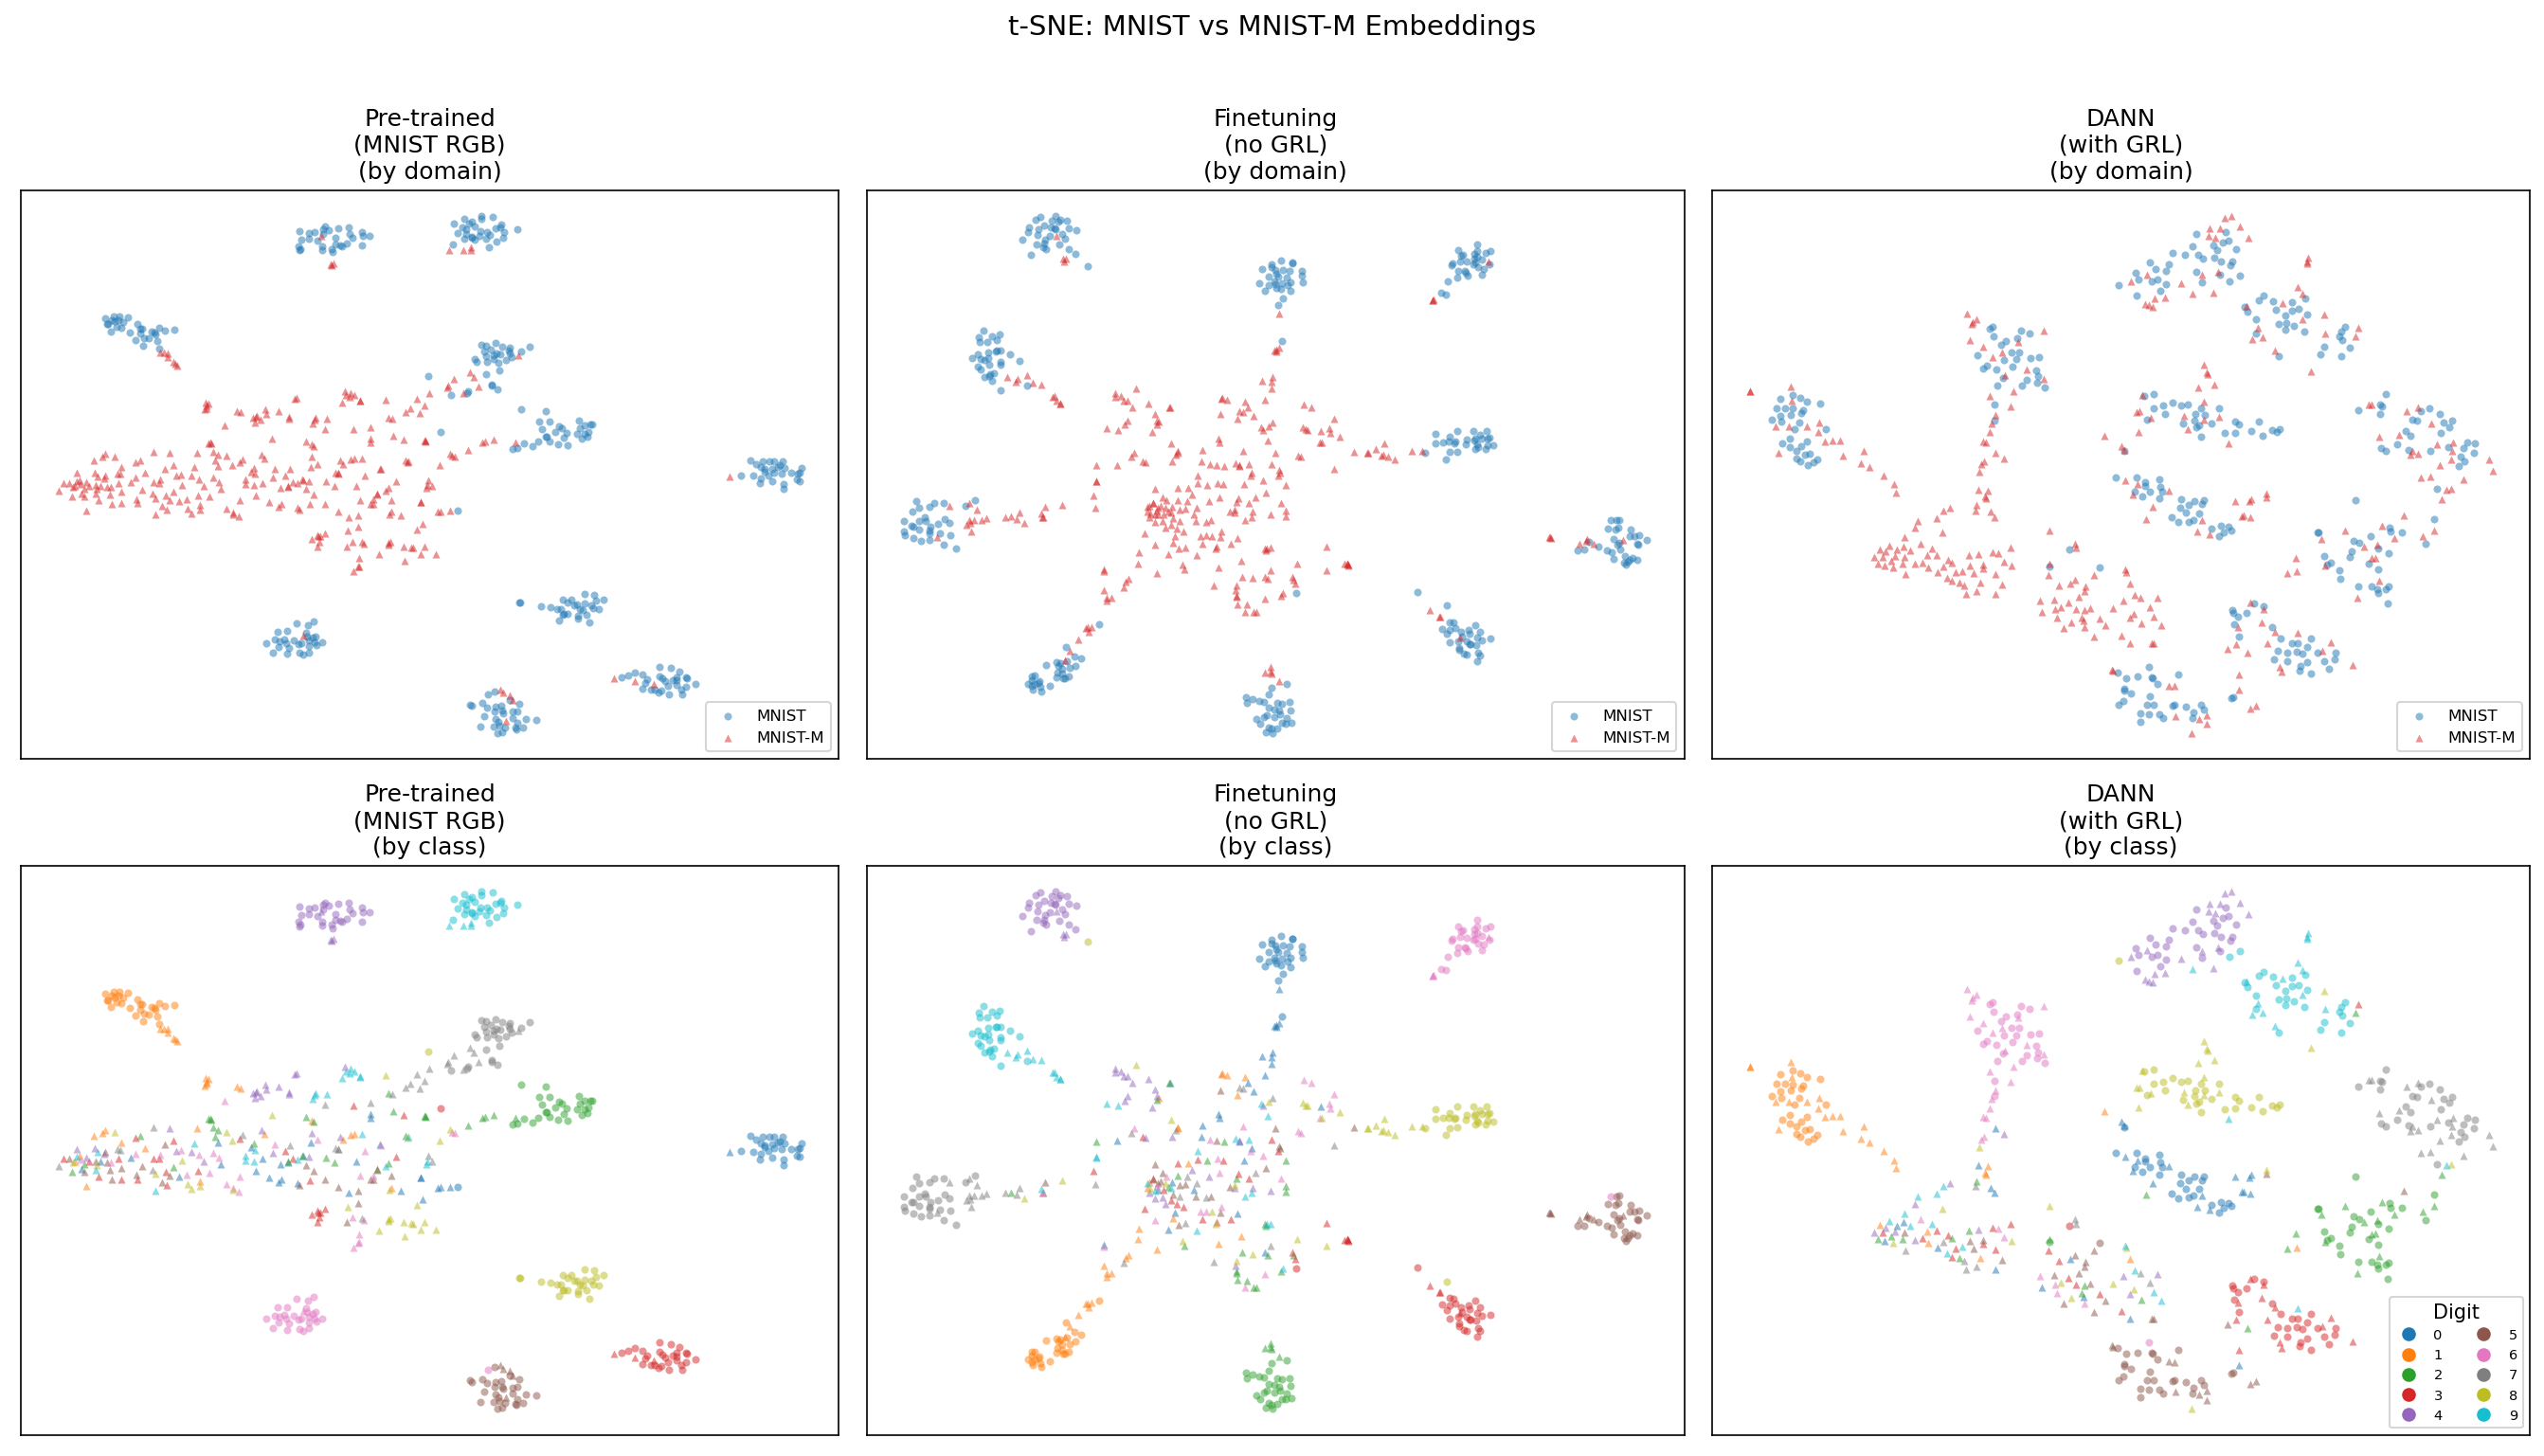
\includegraphics[width=\linewidth]{checkpoints/dann_tsne_comparison.png}
    \caption{t-SNE de \textit{embeddings} de MNIST y MNIST-M en tres momentos: encoder preentrenado, \textit{baseline}, y DANN. Fila superior: por dominio. Fila inferior: por clase.}
    \label{fig:dann_tsne}
\end{figure}

\section{Conclusiones}

INSERTAR CONCLUSIONES

\end{document}